\documentclass[preprint]{elsarticle}
\usepackage[margin=1in]{geometry}
\usepackage{hyperref}
\usepackage{amsmath}
\usepackage{mathrsfs}
\usepackage{float}
\graphicspath{{figures/}}
%\setlength\parindent{0pt}

\DeclareMathOperator{\card}{card}
\DeclareMathOperator{\trc}{trace}
\DeclareMathOperator{\mean}{mean}
\DeclareMathOperator{\bin}{bin}
\DeclareMathOperator{\lns}{lanes}
\DeclareMathOperator{\cnt}{count}

\makeatletter
\def\ps@pprintTitle{%
 \let\@oddhead\@empty
 \let\@evenhead\@empty
 \def\@oddfoot{\centerline{\thepage}}%
 \let\@evenfoot\@oddfoot}
\makeatother


%\usepackage{lineno,hyperref}
%\modulolinenumbers[5]

%\journal{Journal of \LaTeX\ Templates}

%%%%%%%%%%%%%%%%%%%%%%%
%% Elsevier bibliography styles
%%%%%%%%%%%%%%%%%%%%%%%
%% To change the style, put a % in front of the second line of the current style and
%% remove the % from the second line of the style you would like to use.
%%%%%%%%%%%%%%%%%%%%%%%

%% Numbered
%\bibliographystyle{model1-num-names}

%% Numbered without titles
%\bibliographystyle{model1a-num-names}

%% Harvard
%\bibliographystyle{model2-names.bst}\biboptions{authoryear}

%% Vancouver numbered
%\usepackage{numcompress}\bibliographystyle{model3-num-names}

%% Vancouver name/year
%\usepackage{numcompress}\bibliographystyle{model4-names}\biboptions{authoryear}

%% APA style
%\bibliographystyle{model5-names}\biboptions{authoryear}

%% AMA style
%\usepackage{numcompress}\bibliographystyle{model6-num-names}

%% `Elsevier LaTeX' style
\bibliographystyle{elsarticle-num}
%%%%%%%%%%%%%%%%%%%%%%%

\begin{document}

\begin{frontmatter}

\title{Prediction of traffic oscillation instability with spectral analysis of the Aw--Rascle--Zhang model}

%% Group authors per affiliation:
\author[add]{Authors}
\address[add]{address}
%\author{Elsevier\fnref{myfootnote}}
%\address{Radarweg 29, Amsterdam}
%\fntext[myfootnote]{Since 1880.}
%
%%% or include affiliations in footnotes:
%\author[mymainaddress,mysecondaryaddress]{Elsevier Inc}
%\ead[url]{www.elsevier.com}
%
%\author[mysecondaryaddress]{Global Customer Service\corref{mycorrespondingauthor}}
%\cortext[mycorrespondingauthor]{Corresponding author}
%\ead{support@elsevier.com}
%
%\address[mymainaddress]{1600 John F Kennedy Boulevard, Philadelphia}
%\address[mysecondaryaddress]{360 Park Avenue South, New York}

\begin{abstract}
This article will focus on macroscopic second-order models as opposed
to microscopic and mesoscopic frameworks.
\end{abstract}

\begin{keyword}

\end{keyword}

\end{frontmatter}

%\linenumbers

\section{Introduction}

As personal vehicle ownership increases globally, traffic congestion
continues to be a persistent problem. One goal of research in the physics of traffic is to gain a greater understanding of the phenomena, of which proper control would lead to mitigation of congestion. Traffic control strategies such as
ramp metering and variable speed limits are in place today, but improved models of traffic dynamics could lay the foundations for more efficient coordination of
control strategies. 

What constitutes an ``accurate" model often depends on the practitioners' requirements. The model must describe key phenomena in the dynamics of the system under scrutiny so that they can be controlled efficiently. For traffic, a common class of models relies on hydrodynamic theory, modeling vehicular flow in an aggregate manner. However, control schemes are only as reliable as the models on which they are based. Each model can reproduce some features of traffic flow; a challenge of traffic engineering is the selection of the model most appropriate for the application of interest. 

\subsection{First-order models}
The 1950's saw the development of the \textit{Lighthill--Whitham--Richards}
(LWR) model \cite{LW,Richards}, which became the seminal model for aggregate
traffic flow. The dynamics of this first-order scalar hyperbolic conservation law is governed by
\begin{equation}
\rho_t+Q_x=0,
\end{equation}
where $\rho$ is the lineic vehicular density (veh/m), and $Q(\rho)$ is the empirically measured traffic flux (veh/s), also referred to as the fundamental diagram. Numerous phonomenological models exist for $Q(\rho)$,  such as the Greenshields model \cite{Greenshieldsflux}, the Greenberg model \cite{Greenbergflux}, the triangular model, \cite{Newell1993, daganzo1994cell}, etc. The simplicity of the LWR model enabled the formulation of numerical discretization
schemes such as the Godunov scheme \cite{godunov,Osher}, later renamed the cell transmission
model \cite{daganzo1994cell,daganzo1995cell} in the transportation community. 

First-order models have inherent shortcomings, most of which are discussed at length in \cite{Dag_requiem}, such as failure to capture accurately shock structure, light traffic dynamics, and stop-and-go behavior, otherwise known as traffic oscillations. The last phenomenon in particular has attracted increasing attention in transportation research. Jamitons, traffic jams that appear without the presence of a bottleneck, have been reproduced in small experiments \cite{Jamitons2008,Flynn08onjamitons} and explained theoretically
as the result of both particular configurations of the traffic system
\cite{Flynn09self-sustainednonlinear} and
fuzzy fundamental diagrams \cite{Jamitons-multi-valued-fund}. 

%Empirical studies have focused on detecting and quantifying this effect on actual freeways \cite{zielke2008empirical}. Car-following behaviors and lane-changing are often cited as the cause of oscillations \cite{Mauch02freewaytraffic, lanechangin2005,lanechanging2007}. Several approaches have been developed in order to model these empirical facts.

\subsection{First-generation second-order models}
In an effort to refine traffic modeling, Payne and Whitham followed the same approach as in fluid dynamics developed a higher-order model to capture momentum-related features \cite{payne1971models,whitham1974linear}. The \textit{Payne--Whitham} (PW) model consists of a mass conservation equation as in the LWR model,  

\begin{equation}
\rho_t + (\rho v)_x = 0, 
\end{equation}
where $\rho$ and $v$ are the density and velocity, respectively. This is seconded by a momentum equation,
\begin{equation}
v_t+vv_x+\frac{p'\left(\rho\right)}{\rho}\rho_x =\frac{V(\rho)-v}{\tau}+\nu v_{xx} ,
\end{equation}
where the pressure function, $p(\rho)$, is strictly increasing and the equilibrium speed, $V(\rho)$, is nonincreasing. Both are empirically measured and $V(\rho)$ satisfies $Q(\rho) = \rho V(\rho)$. The parameters $\tau$ and $\nu$ are nonnegative, representing the relaxation time and coefficient of viscosity, respectively. This approach, however, has issues in both the derivation of its equations, and its predictions \cite{Dag_requiem}. The PW model relies on the assumption that spacing and speed vary slowly, yielding negligible second and third derivatives for these quantities. This is contradictory with the observations of Newell \cite{Newell} given that the car-following model predicts sharp changes in these quantities. Also, the PW model violates the anisoptropy of traffic flow and can predict negative speeds \cite{Z}.

%Despite the common practice, modeling traffic as a gas is highly unrealistic as fluids feature isotropic propagation of information, while in traffic cars react mainly to downstream conditions. This is incompatible with the PW model since the slope of one of the characteristic curves is greater than cars' speeds. Also, at the upstream end of a jam with low density, traffic would flow in reverse if $\nu\neq0$, which is unrealistic. Finally, gas particles are physically identical whereas drivers have different habits and desired speeds. 

\subsection{Second-generation second-order models}
Despite the pessimism Daganzo expressed in \cite{Dag_requiem} regarding higher-order models inspired by fluid dynamics, Zhang proposed improved models to resolve issues plaguing earlier second-order models. In \cite{Zhang1998}, he proposed a modification of the momentum equation of the PW model to tackle the issue of backward-propagating traffic.
%\begin{equation}
%v_t+vv_x+\rho\left(V'\left(\rho\right)\right)^{2}\rho_x=\frac{V\left(\rho\right)-v}{\tau},
%\end{equation}
%where $\rho V'\left(\rho\right)$ represents the information
%propagation speed in traffic. 
Soon after, Aw and Rascle \cite{AR} presented a model with the following momentum equation:
\begin{equation}
\frac{\partial\left(v+p\left(\rho\right)\right)}{\partial t}+v\frac{\partial\left(v+p\left(\rho\right)\right)}{\partial x}=\frac{V(\rho)-v}{\tau}.
\end{equation}
Including the pressure term, $p(\rho)$, in a convective derivative guarantees no information travels faster than the speed of the cars. Aw and Rascle demonstrated in \cite{AR} that ``with a suitable choice of function $p$," the above class of models avoids inconsistencies of earlier second-order models. Zhang proposed in \cite{Z} the same model with $p(\rho) = -V(\rho)$. With this choice of $p(\rho)$, the model is referred to as the \textit{Aw--Rascle--Zhang} (ARZ) model.

This model has since been thoroughly studied. The work in
\cite{AR} concluded that a relaxation term accounting for traffic
equilibrium was needed so the speed of cars would be determined by
the fundamental diagram and not the initial data. Rascle later proved in \cite{R_improved} that the relaxed model converges towards the LWR model as $\tau \rightarrow 0$. The first ARZ model required a fundamental diagram extended to negative and maximum speeds, and zero and maximum densities so as to guarantee
solutions to the Riemann problem and stability with low densities \cite{Lebacque2007}. In \cite{HybridLagrangian2007}, 
discretization enabled extension of the AR model to a network setup with junctions and traffic lights. With an extended fundamental diagram, any Riemann problem for the ARZ model can be solved, allowing for a Godunov descretization scheme and numerical comparison
in which the ARZ model fits real data better than the LWR model \cite{GodunovARZ}.

%The ARZ model now has a legacy that started with the extended ARZ model \cite{lebacque2007generic}. An extension was presented in \cite{berthelin2008model} as a pressure-less limit of the AR model where drivers will not significantly slow down if the congestion is not heavy. More recently a generalized model proposed in \cite{Fan} corrects the fact that, in the ARZ model, several maximum densities co-exist, seemingly contradictory to the fact that this quantity is uniquely determined by the characteristics of the freeway.  

\subsection{Models appropriate for control}
It is noted in \cite{Fan} that for congested regimes, the 
LWR model tends to offer a slightly better fit than the ARZ model with respect to empirical measurements but is outperformed for low densities. Ideally we would use a model suitable for all regimes so as to establish generic control strategies for traffic. Because such a model does not exist, we choose instead to develop the ARZ model linearized around arbitrary nominal conditions. Certain second-order models, including the ARZ model, realistically account for traffic oscillations in dense traffic \cite{Greenberg_congestionredux}. Laplace transform and spectral analysis are powerful tools for control problems, providing a simple yet holistic representation of a system. In this regard,
it is important to have a model that predicts oscillatory phenomena. Behavioral models such as in \cite{Newell}, and more recently
\cite{Chen2012}, depict in a detailed fashion the effects of car-following
and lane-changing on freeway dynamics, effects often cited as the cause of oscillations \cite{Mauch02freewaytraffic, lanechangin2005,lanechanging2007}. However, second-order macroscopic models are most suited for our method. 

%Recent data driven approaches \cite{Zheng2011} that attempt to model spectral features of traffic using wavelet transform are also not suitable. They are mostly heuristic in that they do not focus on the dynamics core to the system.

\subsection{Similarities with Saint-Venant equations}
Our control analysis of the ARZ equations is strongly
inspired by the pioneering analysis of the Saint-Venant equations in \cite{litrico2009modeling}. The equations are as follows:
\begin{align}
T\frac{\partial y}{\partial t}+\frac{\partial q}{\partial x}&=0, \\
\frac{\partial v}{\partial t}+v\frac{\partial v}{\partial x}+g\frac{\partial y}{\partial x}&=g\left(S_{b}-S_{f}\right),
\end{align}
where $v$ is the fluid velocity in a canal, $q$ the flux, $T$ the top width, $y$ the water height, $S_f$ the friction slope, and $S_b$ the bed slope. Note the structural similarity to the ARZ equations. In the equilibrium regime, the term $S_{b}-S_{f}\left(x,t\right)$ is zero under uniform flow, making it analogous to the relaxation term $\frac{V(\rho)-v}{\tau}$, defined to be zero at the equilibrium. Linearizing this system around an equilibrium point enables the use of spectral methods to design efficient control strategies for canals \cite{Litricoapplic}. Approximations for the low frequency domain decompose the transfer matrix into a combination of delay and integration components, allowing for design of efficient PI controllers while enabling a simpler theoretical analysis of hydraulic systems.

\subsection{Approach and contributions}
This article adapts the corresponding spectral framework of \cite{litrico2009modeling} to the analogous ARZ equations so as to achieve a two-fold objective:

\begin{itemize}
\item We aim to develop strategies that enforce ease of use of the ARZ model. Analytical solutions to these non-linear equations are difficult to derive but linearization facilitates design of efficient control schemes with multiple inputs and outputs. We must also be careful in the formulation of boundary conditions, to guarantee the well-posedness of the problem.
\item We assess the fit quality of the model by comparing its output with actual data collected as part of the NGSIM project. 
\end{itemize}

The contributions of this article are as follows:

\begin{itemize}
\item \textit{Modeling}: We derive the characteristic form by linearization and diagonalization of the ARZ model. This form highlights important features of the model, leading to the definition of an analogue of the Froude number from hydrodynamics \cite{litrico2009modeling}, separating free-flow and congested regimes.  

\item \textit{Spectral analysis}: From the charateristic form we derive the spectral form. Time domain responses derived from the spectral transfer matrices show that the linearized system is unstable in the free-flow regime and accounts for nonlinear wave propagation, giving rise to jamitons. These waves occur for an entire set of values of velocity, density, and flux and lead the linearized system away from its equilibrium point in the free-flow regime. 

\item \textit{Numerical vaildation}: A numerical experiment using NGSIM data is conducted to verify that linearization does not destroy realistic properties of the ARZ model. Previous studies also using NGSIM data to assess predictions of second-order models focused on averaged errors and only displayed predictions at a couple of points along the freeway \cite{GodunovARZ,Fan}. Here we show an entire map of the states and conduct model assessment in a holistic manner, providing a complete analysis of the strengths and weaknesses of the model to be used for control. Our estimation procedure, unlike \cite{Fan}, does not rely on any assumption about the typical vehicle length or the safety distance factor. Additionally, no discretization scheme is needed and no grid size condition needs to be fulfilled. This procedure proves that the linearized model successfully accounts for traffic oscillations and also provides simple and consistent methods to calibrate the relaxation time, $\tau$.
\end{itemize}

\subsection{Organization of the article}
The rest of this article is organized as follows. In Section 2 we present the characteristic form of the ARZ model in several state variables, leading to the derivation of the spectral form of the flux and velocity system in section 3. We focus on these states in particular as they are the most easily observed and controlled in traffic. Properties of the spectral form in the two flow regimes are also analyzed. Section 4 focuses on numerical analysis. We present estimation procedures for $(v,q,\rho)$ and the model parameters, comparing empirical estimates with numerical predictions of the linearized model. We use Fast Fourier Transform to turn the spectral model into a prediction tool.


\section{The ARZ model}

%\begin{itemize}
%\item physical description of ARZ model + usual form
%\item $(v, q)$ form, well-posedness 
%\end{itemize}

In this article we consider the ARZ model with relaxation term. The model is reproduced below: 
\begin{align} 
\rho_t + (\rho v)_x &= 0, \label{ARZ1} \\
(v - V(\rho))_t + v(v - V(\rho))_x &=\dfrac{V(\rho) - v}{\tau} \label{ARZ2},
\end{align}
where $\rho$ is the density, $v$ is the velocity, $\tau$ is the relaxation time, and $V(\rho) = Q(\rho)/\rho$ is the equilibrium velocity profile, where $Q(\rho)$ is the density-flow relation given by the fundamental diagram. Without the relaxation term cars never reach the maximum allowable speed \cite{R_improved}. Note that at the equilibrium velocity this term is zero. 

In vector form the ARZ model is
\begin{equation} \label{ARZrhov}
\begin{pmatrix}
\rho \\ v
\end{pmatrix}_t
+ \begin{pmatrix}
v & \rho \\
0 & v + \rho V' (\rho)
\end{pmatrix}
\begin{pmatrix}
\rho \\ v
\end{pmatrix}_x = 
\begin{pmatrix}
0 \\ \dfrac{V(\rho) - v}{\tau}
\end{pmatrix}.
\end{equation}

With the appropriate variable change, we can rewrite the model in the denisty-flow and velocity-flow forms, the latter of which is most useful to us for practical control purposes. Using the flow relation $q = \rho v$ and \eqref{ARZrhov}, the density-flow form is
\begin{equation} \label{ARZrhoq}
\begin{pmatrix}
\rho \\ q
\end{pmatrix}_t
+ \begin{pmatrix}
0 & 1 \\
-\frac{q}{\rho} \left(\frac{q}{\rho} + \rho V'(\rho) \right) & 2\frac{q}{\rho} + \rho V'(\rho) 
\end{pmatrix}
\begin{pmatrix}
\rho \\ q
\end{pmatrix}_x = 
\begin{pmatrix}
0 & 0 \\ 
\frac{V(\rho)}{\tau} & -\frac{1}{\tau}
\end{pmatrix} 
\begin{pmatrix}
\rho \\ q
\end{pmatrix}.
\end{equation}

In the same manner we arrive at the velocity-flow form,
\begin{equation} \label{ARZvq}
\begin{pmatrix}
v \\ q
\end{pmatrix}_t
+ \begin{pmatrix}
v + \frac{q}{v} V'\left(\frac{q}{v}\right) & 0 \\
\frac{q}{v} \left( v + \frac{q}{v} V'\left(\frac{q}{v}\right)\right) & v
\end{pmatrix}
\begin{pmatrix}
v \\ q
\end{pmatrix}_x = 
\dfrac{1}{\tau}
\begin{pmatrix}
V\left( \frac{q}{v}\right) - v \\
\frac{q}{v}V\left( \frac{q}{v}\right) - q
% \dfrac{V\left( \frac{q}{v}\right) - v}{\tau} \\ 
% \dfrac{\frac{q}{v}V\left( \frac{q}{v}\right) - q}{\tau}
\end{pmatrix}.
\end{equation}

\subsection{Linearization}
We are interested in small deviations, $(\tilde{\rho}(x,t), \tilde{v}(x,t))$, from the nominal profile. Consider the nominal solution $(\rho^*(x),v^*(x))(V(\rho^*) = v^*)$ satisfying $v_t = \rho_t = 0$. Then \eqref{ARZrhov} becomes
\begin{align}
v^* \frac{d\rho^*}{dx} + \frac{dv^*}{dx}\rho^* = 0, \\
\left( v^* + \rho^* V'( \rho^*) \right)\frac{dv^*}{dx} = \dfrac{V(\rho^*) - v^*}{\tau} = 0.
\end{align}
Then we must have $v^*_x=\rho^*_x=0$, so the solution is uniform along the road. 

Linearizing the ARZ model \eqref{ARZrhov} around the nominal solution described above, we obtain
\begin{equation} \label{rhovlin}
\begin{pmatrix}
\tilde{\rho} \\ \tilde{v}
\end{pmatrix}_t
+ \begin{pmatrix}
v^* & \rho^* \\
0 & v^* + \rho^* V' ( \rho^*) 
\end{pmatrix}
\begin{pmatrix}
\tilde{\rho} \\ \tilde{v}
\end{pmatrix}_x = 
\begin{pmatrix}
0 & 0 \\
\dfrac{V' (\rho^*)}{\tau} & -\frac{1}{\tau}
\end{pmatrix}
\begin{pmatrix}
\tilde{\rho} \\ \tilde{v}
\end{pmatrix}
\end{equation}

Similarly for the density-flow system \eqref{ARZrhoq}, we linearize around the equilibrium $(\rho^*, q^*)(\rho^*V(\rho^*) = q^*)$ with deviations $(\tilde{\rho}(x,t), \tilde{q}(x,t))$. The linearized system is as follows 
\begin{equation} \label{rhoqlin}
\begin{pmatrix}
\tilde{\rho} \\ \tilde{q}
\end{pmatrix}_t
+ \begin{pmatrix}
0 & 1 \\
\alpha^* \beta^* & \alpha^* - \beta^* 
\end{pmatrix}
\begin{pmatrix}
\tilde{\rho} \\ \tilde{q}
\end{pmatrix}_x = 
\begin{pmatrix}
0 & 0 \\
\delta & \sigma
\end{pmatrix}
\begin{pmatrix}
\tilde{\rho} \\ \tilde{q}
\end{pmatrix},
\end{equation}
where $\alpha^* = \frac{q^*}{\rho^*}$, $\beta^* = -\frac{q^*}{\rho^*} - \rho^* V'(\rho^*)$, $\delta = \dfrac{V(\rho^*)+\rho^*V'( \rho^*)}{\tau}$, and $\sigma = -\dfrac{1}{\tau}$.

Finally, for the velocity-flow system, 
\begin{equation} \label{vqlin}
\begin{pmatrix}
\tilde{v} \\ \tilde{q}
\end{pmatrix}_t
+ \begin{pmatrix}
v^* + \frac{q^*}{v^*} V'\left(\frac{q^*}{v^*}\right) & 0 \\
\frac{q^*}{v^*} \left( v^* + \frac{q^*}{v^*} V'\left(\frac{q^*}{v^*}\right)\right) & v^*
\end{pmatrix}
\begin{pmatrix}
\tilde{v} \\ \tilde{q}
\end{pmatrix}_x = 
\begin{pmatrix}
-\dfrac{(v^*)^2+q^*V'\left(\frac{q^*}{v^*}\right)}{(v^*)^2 \tau} & \dfrac{V'\left(\frac{q^*}{v^*}\right)}{v^* \tau} \\
-\dfrac{q^*\left((v^*)^2 + q^*V'\left(\frac{q^*}{v^*}\right)\right)}{(v^*)^3 \tau}  & \dfrac{q^*V'\left(\frac{q^*}{v^*}\right)}{(v^*)^2 \tau}
\end{pmatrix}
\begin{pmatrix}
\tilde{v} \\ \tilde{q}
\end{pmatrix}.
\end{equation}

\subsection{Characteristic form}
We rewrite the model in the characteristic form by diagonalizing the linearized equations. 
%We can rewrite \eqref{rhovlin} in diagonal form. The eigenvalues of $A$ are 
%\begin{align}
%\lambda_1 &= v^*, \\
%\lambda_2 &= v^* + \rho^* V'( \rho^*).
%\end{align}
We begin with the density-flow system. Standard algebraic manipulations of the equations in \eqref{rhovlin} lead to:
\begin{equation}
\begin{pmatrix}
\zeta_1 \\ \zeta_2
\end{pmatrix}_t
+ \begin{pmatrix}
\lambda_1 & 0 \\
0 & \lambda_2 
\end{pmatrix}
\begin{pmatrix}
\zeta_1 \\ \zeta_2
\end{pmatrix}_x
= \begin{pmatrix}
-\frac{1}{\tau} & 0 \\
-\frac{1}{\tau} & 0
\end{pmatrix}
\begin{pmatrix}
\zeta_1 \\ \zeta_2
\end{pmatrix},
\end{equation}
where $\zeta_1 = \tilde{v} - V'( \rho^* )\tilde{\rho}$ and $\zeta_2 = \tilde{v}$ are the Riemann invariants of the $(\rho, v)$ system, and $\lambda_1 = v^*$ and $\lambda_2 = v^* + \rho^* V'( \rho^*)$ are the eigenvalues. Note that $V'( \rho^*) < 0$ so $\lambda_2 \leq \lambda_1 = v^*$. Therefore this is consistent with the physical dynamics of the system as no waves travel faster than the equilibrium vehicle speed. 

We proceed in the same manner as above to diagonalize the $(\rho,q)$ system \eqref{rhoqlin}. The diagonal form is
\begin{equation} \label{rhoqlindiag}
\begin{pmatrix}
\chi_1 \\ \chi_2
\end{pmatrix}_t 
+ \begin{pmatrix}
\lambda_1 & 0 \\
0 & \lambda_2
\end{pmatrix}
\begin{pmatrix}
\chi_1 \\ \chi_2
\end{pmatrix}_x
= \begin{pmatrix}
-\frac{1}{\tau} & 0 \\
-\frac{1}{\tau} & 0
\end{pmatrix}
\begin{pmatrix}
\chi_1 \\ \chi_2
\end{pmatrix},
\end{equation}
where $\chi_1 = -\lambda_2 \tilde{\rho} + \tilde{q}$ and $\chi_2 = -\lambda_1 \tilde{\rho} + \tilde{q}$ are the characteristic variables in the $(\rho,q)$ system and the eigenvalues $\lambda_1$ and $\lambda_2$ are the same as in the density-velocity system due to the relation $q^* = \rho^*v^*$. 

Diagonalization of the velocity-flow system is more involved. Letting $\xi(x,t) = (\tilde{v}, \tilde{q})^T$, we can rewrite \eqref{vqlin} as
\begin{equation} \label{vqlinxi}
\eta_t + A\eta_x = B\eta.
\end{equation}
The eigenvalues of $A$ are $\lambda_1 = v^*$ and $\lambda_2 = v^* + \frac{q^*}{v^*} V'\left(\frac{q^*}{v^*}\right)$, consistent with the previous systems. Then $A$ can be diagonalized as follows
\begin{align}
A &= XDX^{-1}, \\
X &= \begin{pmatrix}
0 & \lambda_2-\lambda_1 \\
1 & \rho^*\lambda_2
\end{pmatrix}, \\
D &= \begin{pmatrix}
\lambda_1 & 0 \\
0 & \lambda_2
\end{pmatrix},\\
X^{-1} &= \begin{pmatrix}
\dfrac{\rho^*\lambda_2}{\lambda_1 - \lambda_2} & 1 \\
-\dfrac{1}{\lambda_1 - \lambda_2} & 0
\end{pmatrix}.
\end{align}

Define $\gamma(x,t) := X\eta(x,t)$. Hence \eqref{vqlinxi} can be rewritten as
\begin{equation} 
\gamma_t + \begin{pmatrix}
\lambda_1 & 0 \\
0 & \lambda_2
\end{pmatrix} \gamma_x = \begin{pmatrix}
-\frac{1}{\tau} & 0 \\
-\frac{1}{q^* \tau} & 0
\end{pmatrix} \gamma
\end{equation}
where 
\begin{equation}
\gamma = \begin{pmatrix}
\frac{\rho^*\lambda_2}{\lambda_1 - \lambda_2}\tilde{v} + \tilde{q} \\ 
-\frac{1}{\lambda_1 - \lambda_2}\tilde{v} 
\end{pmatrix}. 
\end{equation}

Let $\xi = (\xi_1, \xi_2)^T = (\chi_1, -q^*\chi_2)^T$. Then we have
\begin{equation} \label{vqlindiag}
\begin{pmatrix}
\xi_1 \\ \xi_2
\end{pmatrix}_t + \begin{pmatrix}
\lambda_1 & 0 \\
0 & \lambda_2
\end{pmatrix} \begin{pmatrix}
\xi_1 \\ \xi_2
\end{pmatrix}_x = \begin{pmatrix}
-\frac{1}{\tau} & 0 \\
-\frac{1}{\tau} & 0
\end{pmatrix} \begin{pmatrix}
\xi_1 \\ \xi_2
\end{pmatrix},
\end{equation}
and
\begin{equation} \label{eq:Riemannzeta}
\begin{pmatrix}
\xi_1 \\ \xi_2
\end{pmatrix} = \begin{pmatrix}
\dfrac{\rho^*\lambda_2}{\lambda_1 - \lambda_2}\tilde{v} + \tilde{q} \\ 
\dfrac{q^*}{\lambda_1 - \lambda_2}\tilde{v} 
\end{pmatrix} = 
\begin{pmatrix}
\dfrac{\rho^*\lambda_2}{\lambda_1-\lambda_2} & 1\\
\dfrac{\rho^*\lambda_1}{\lambda_1-\lambda_2} & 0
\end{pmatrix} \begin{pmatrix}
\tilde{v} \\ \tilde{q} 
\end{pmatrix}
\end{equation}

\subsection{The Traffic Froude Number}
In fluid mechanics, the Froude number is a dimensionless number which delineates the boundary between flow regimes \cite{Sturm, litrico2009modeling}. Using the eigenvalues of the system in the characteristic form, we are able to define a useful analog to this number.
Since $V(\rho)$ is nonincreasing function, we have $V'(\rho^*) \leq 0$. Thus there are two flow regimes, one where $\lambda_1 \lambda_2 < 0$ and one characteristic curve travels downstream, and one where $\lambda_1 \lambda_2 > 0$ and both characteristic curves travel upstream. 

We define the Traffic Froude Number (TFN) as
\begin{equation}
F = \dfrac{\rho^*V'( \rho^*)}{v^*}.
\end{equation} 
Then we have
\begin{equation*}
\begin{cases}
F > 1 &\Rightarrow |\rho^*V'(\rho^*)| > v^* \quad \Rightarrow \lambda_2  <0 \\
F < 1 &\Rightarrow |\rho^*V'(\rho^*)| < v^* \quad \Rightarrow \lambda_2 > 0
\end{cases}.
\end{equation*}
Note also that $\lambda_2 = v^* + \rho^* V'( \rho^*) = \dfrac{Q(\rho^*)}{\rho^*} + \dfrac{\rho^*Q'(\rho^*)-Q(\rho^*)}{\rho^*} = Q'(\rho^*)$. Hence the system is in free-flow when $F<1$ and congestion when $F>1$. In hydrodynamics these regimes are referred to as the supercritical and subcritical regimes, respectively \cite{litrico2009modeling}.


\section{Spectral analysis of the linearized ARZ model}
We consider only the $(v,q)$ system for the frequency domain analysis for practical control purposes as described above.
\subsection{State-transition matrix}
Taking the Laplace transform of the diagonalized form \eqref{vqlindiag} we obtain 
\begin{equation}
\dfrac{\partial \hat{\zeta} (x,s)}{\partial x} = \mathscr{A}(s)\hat{\zeta}(x,s) + \mathscr{B}\zeta(x,t=0^-),
\end{equation}
where $\mathscr{A}(s) = A^{-1}(B - sI)$ and $\mathscr{B} = -A^{-1}$. 
The general solution to this ordinary differential equation is 
\begin{equation}
\hat{\zeta}(x,s) = \Phi(x,s)\hat{\zeta}(0,s) +  \Phi(x,s) \int^x_0 \Phi(\nu,s)^{-1} \mathscr{B} \zeta(\nu,0^-)\text{d} \nu,
\end{equation}
where $\Phi(x,s) = e^{\mathscr{A}(s)x}$ is the state-transition matrix. Assuming zero initial conditions we have 
\begin{equation} \label{TFRiemann}
\hat{\zeta}(x,s) = \Phi(x,s)\hat{\zeta}(0,s).
\end{equation}

To compute the exponential we diagonalize the matrix as 
\begin{equation}
\mathscr{A}(s) = \mathscr{X}(s)\mathscr{D}(s)\mathscr{X}^{-1}(s)
\end{equation} 
where  
\begin{align}
\mathscr{X}(s) &= \begin{pmatrix}
0 & \dfrac{\lambda_2 - (\lambda_1 - \lambda_2) \tau s}{\lambda_1} \\
1 & 1
\end{pmatrix}, \\
\mathscr{D}(s) &= \begin{pmatrix}
-\frac{s}{\lambda_2} & 0 \\
 0 & -\frac{1+\tau s}{\tau \lambda_1}
\end{pmatrix}.
\end{align}
Hence
\begin{equation}
\Phi(x,s) =  \mathscr{X}^{-1}(s)e^{\mathscr{D}(s)x}\mathscr{X}(s) =
\begin{pmatrix}
\phi_{11}(x,s) & \phi_{12}(x,s) \\ 
\phi_{21}(x,s) & \phi_{22}(x,s)
\end{pmatrix},
\end{equation}
with
\begin{subequations} \label{TFv0q0tovxqx}
\begin{align}
\phi_{11} &= e^{-\frac{x}{\tau \lambda_1}}e^{-\frac{x}{\lambda_1}s}, \\ 
\phi_{12} &= 0, \\
\phi_{21} &= \dfrac{\lambda_1 \left( e^{-\frac{x}{\tau \lambda_1}}e^{-\frac{x}{\lambda_1}s} - e^{-\frac{x}{\lambda_2}s}\right)}{\lambda_2 - \tau (\lambda_1 - \lambda_2)s}, \\
\phi_{22} &= e^{-\frac{x}{\lambda_2}s}.
\end{align}
\end{subequations}
\subsection{Free-flow case}
Consider the system in the free-flow regime. From \eqref{vqlindiag} we see that $\zeta_1$ travels with characteristic speed $\lambda_1$ and $\zeta_2$ with characteristic speed $\lambda_2$. In the free-flow regime we have $\lambda_1 \geq \lambda_2 > 0$, hence two boundary conditions are needed, both at the upstream boundary. A plot of the characteristics is shown in Figure \ref{fig:supercr}.

\begin{figure}[H] 
\centering
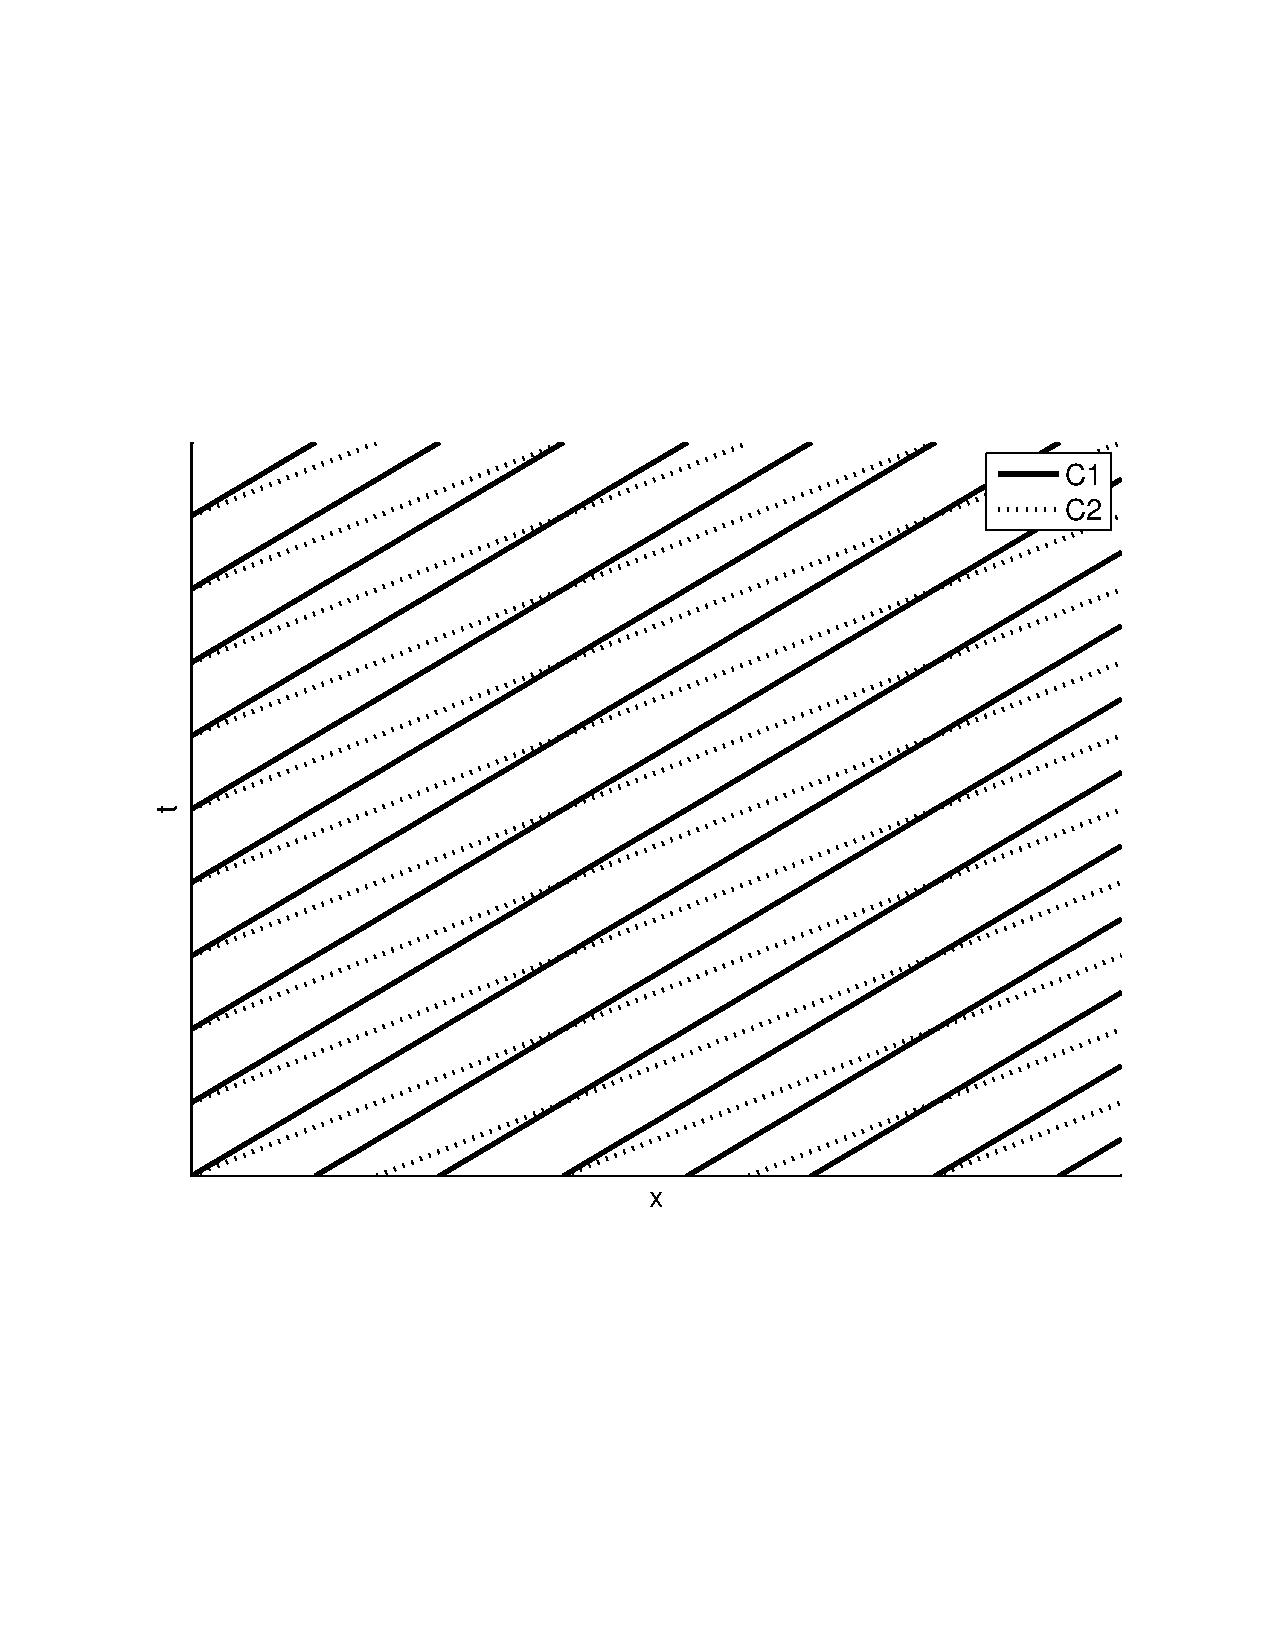
\includegraphics[trim= 0mm 75mm 0mm 70mm, width = 90mm]{supercr}
\caption{Illustration of the characteristics for supercritical flow, $\lambda_1 \geq \lambda_2 > 0$.}
\label{fig:supercr}
\end{figure}

With $\zeta_1 (0,t)$ and $\zeta_2 (0,t)$ as the inputs and $\zeta_1(L,t)$ and $\zeta_2(L,t)$ as the outputs, the distributed transfer matrix is exactly the state-transition matrix $\Phi(x,s)$.\\

Using \eqref{eq:Riemannzeta}, we can write

\begin{equation}
\begin{pmatrix}
\widetilde{v}(x,s) \\ \widetilde{q}(x,s)
\end{pmatrix} = \underbrace{ \begin{pmatrix}
\dfrac{\rho^*\lambda_2}{\lambda_1-\lambda_2} & 1\\
\dfrac{\rho^*\lambda_1}{\lambda_1-\lambda_2} & 0
\end{pmatrix}^{-1} \Phi(x,s) 
\begin{pmatrix}
\dfrac{\rho^*\lambda_2}{\lambda_1-\lambda_2} & 1\\
\dfrac{\rho^*\lambda_1}{\lambda_1-\lambda_2} & 0
\end{pmatrix} }_\text{$\Psi (x,s)$} \begin{pmatrix}
\widetilde{v}(0,s) \\ \widetilde{q}(0,s)
\end{pmatrix}
\end{equation}
with
\begin{subequations}
\begin{align}
\psi_{11}(x,s) &=\left(e^{-\frac{x}{\lambda_{1}\tau}}e^{-\frac{x}{\lambda_{1}}s}-e^{-\frac{x}{\lambda_{2}}s}\right)\frac{\alpha}{s+\alpha}+e^{-\frac{x}{\lambda_{2}}s}, \\
\psi_{12}(x,s)&=-\frac{1}{\rho^* \tau}\left(e^{-\frac{x}{\lambda_{1}\tau}}e^{-\frac{x}{\lambda_{1}}s}-e^{-\frac{x}{\lambda_{2}}s}\right)\frac{1}{s+\alpha}, \\
\psi_{21}(x,s)&=-\rho^{*} \tau\left(e^{-\frac{x}{\lambda_{1}\tau}}e^{-\frac{x}{\lambda_{1}}s}-e^{-\frac{x}{\lambda_{2}}s}\right)\frac{\alpha s}{s+\alpha}, \\
\psi_{22}(x,s)&=-\left(e^{-\frac{x}{\lambda_{1}\tau}}e^{-\frac{x}{\lambda_{1}}s}-e^{-\frac{x}{\lambda_{2}}s}\right)\frac{\alpha}{s+\alpha}+e^{-\frac{x}{\lambda_{1}\tau}}e^{-\frac{x}{\lambda_{1}}s}.
\end{align}
\end{subequations}

where $\alpha = -\dfrac{\lambda_2}{\tau(\lambda_1 - \lambda_2)}$. 

\subsubsection{Bode plots}

We generate Bode plots using the following parameters taken from \cite{Hofleitner}: $q_{max}$ = 1300 veh/h, $\rho_{max}$ = 0.1 veh/m, and $L$ = 100 m: The Greenshields Hamiltonian, $Q( \rho) = 4 \frac{q_{max}}{\rho_{max}^2}\rho (\rho_{max} - \rho)$, is used to approximate the fundamental diagram. For inhomogenous second-order models, the relaxation time, $\tau$, falls in the range of about 14-60 seconds \cite{Fan}. A relaxation time of $\tau$ = 15 s is used for the following simulations. We simulate for $\rho^* = 0.01$. \\

The Bode plots for the physical variables are display on Figure ~\ref{fig:Magn_phase_physx} and Figure \ref{Magn_spatial_physx}. For the Riemann invariants only $\phi_{21}(x,s)$ and $\phi_{22}(x,s)$ are represented on Figure \ref{fig:Magn_phase_diag} and Figure \ref{Magn_spatial_diag} ($\phi_{11}(x,s)$ and $\phi_{12}(x,s)$ are only delay functions).

\begin{figure}
\centering
\begin{tabular}{cc}
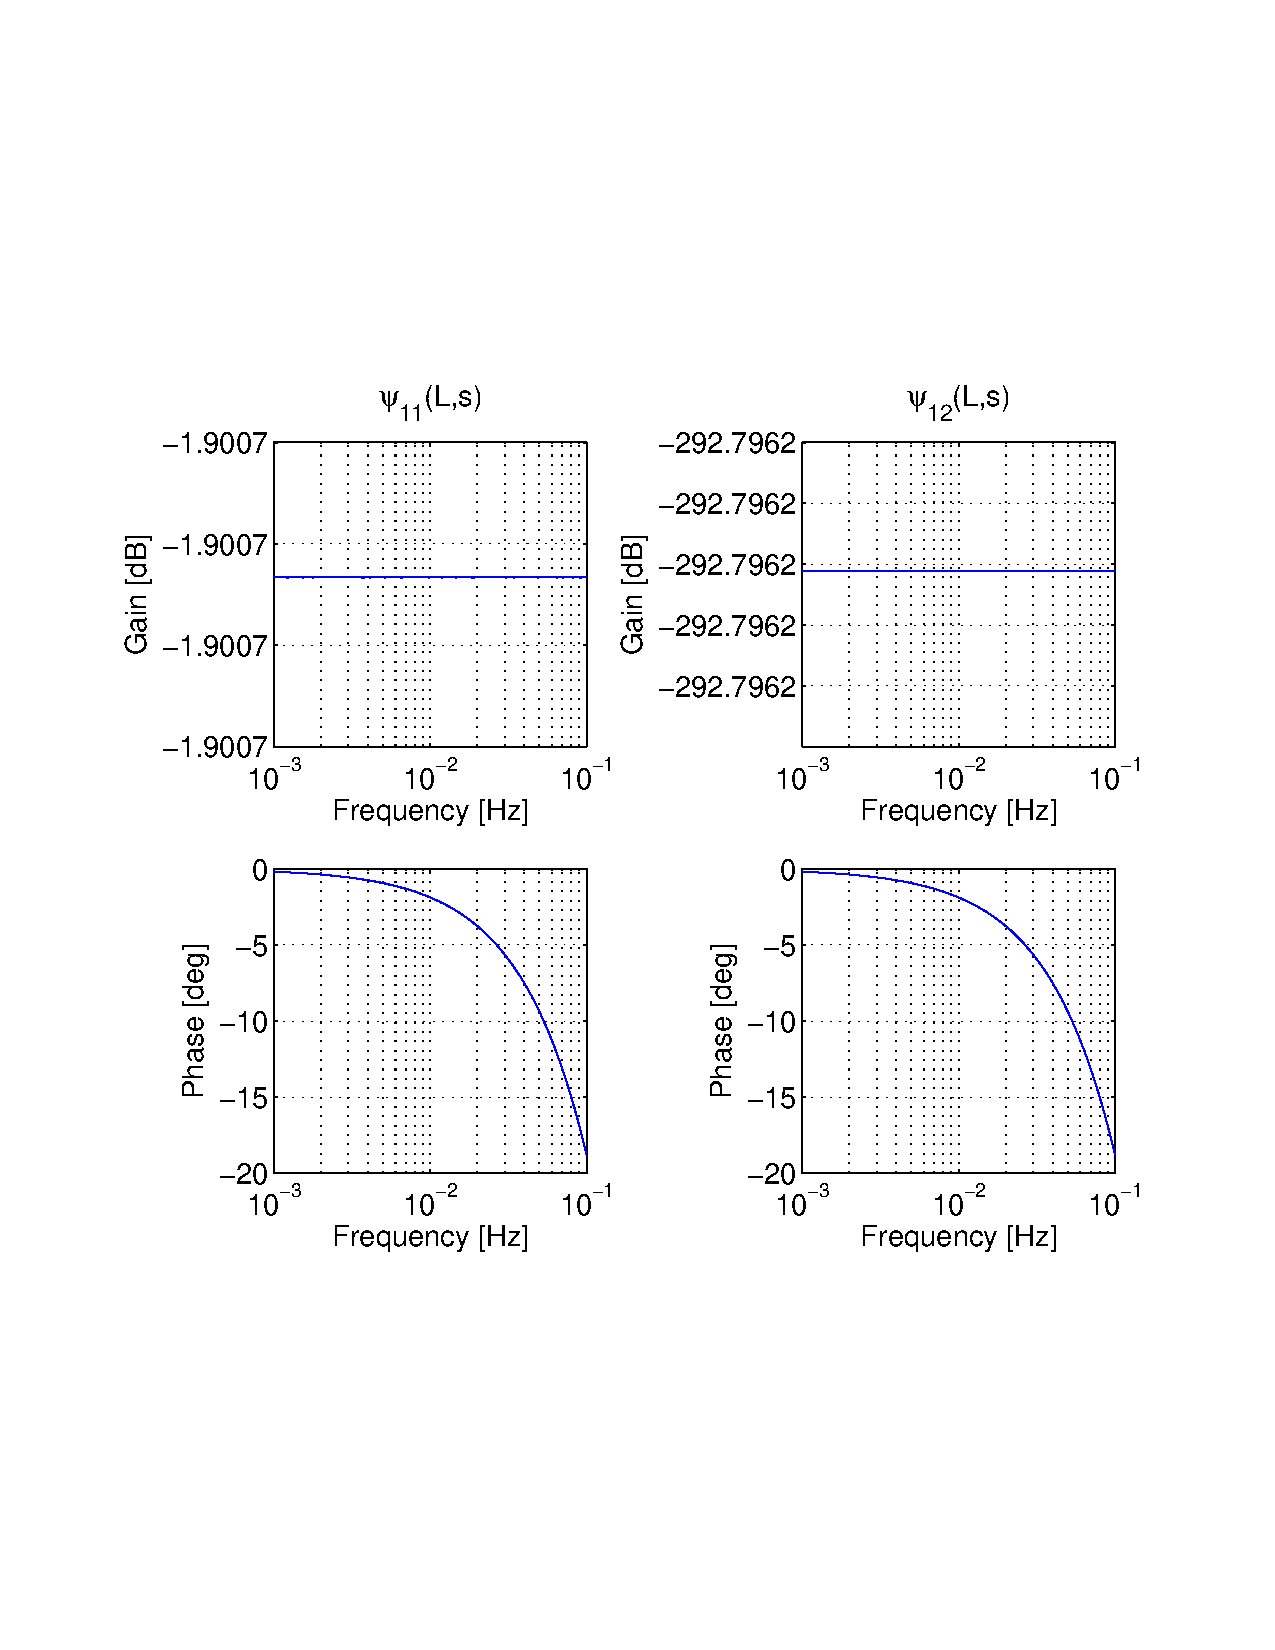
\includegraphics[trim = 0mm 60mm 0mm 60mm, width=8cm]{IOv_-3to-1}
& 
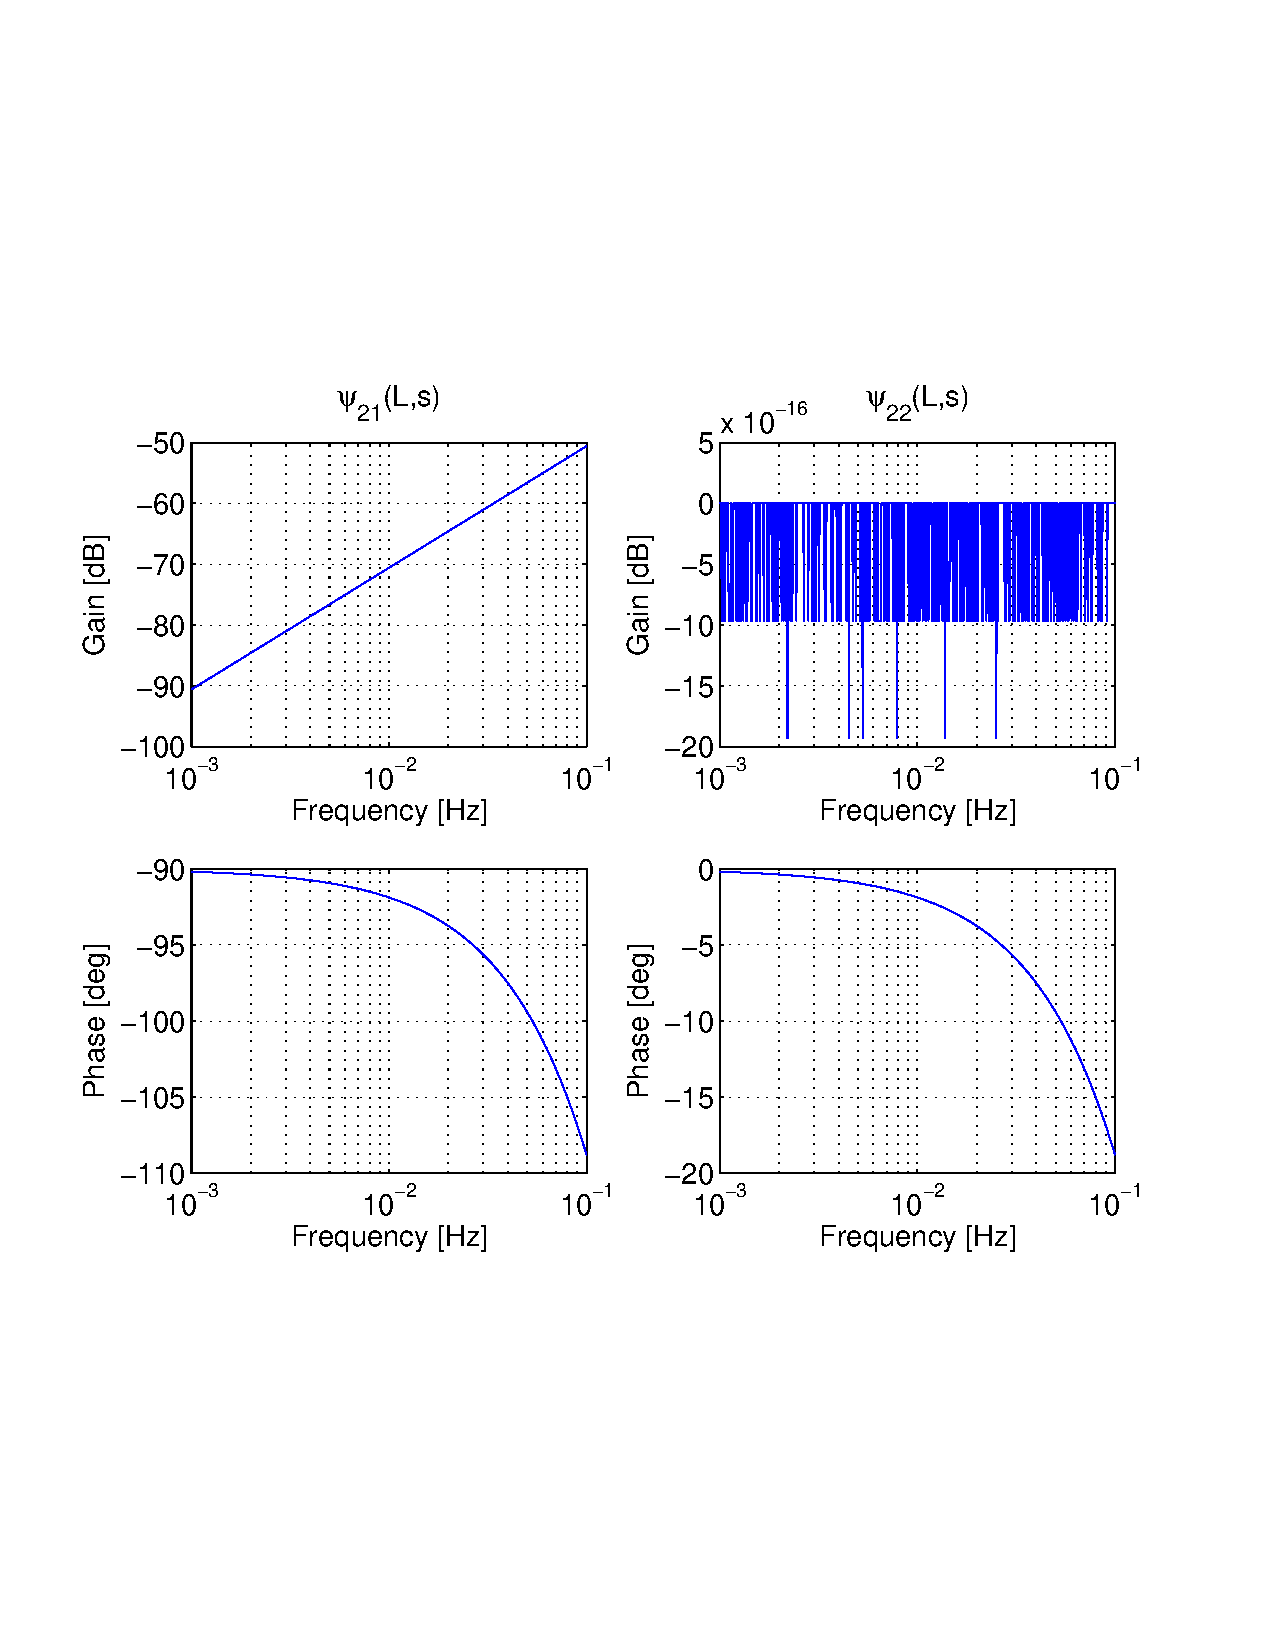
\includegraphics[trim = 0mm 60mm 0mm 60mm, width=8cm]{IOq_-3to-1}
\tabularnewline
\end{tabular}
\caption{
Magnitude and phase bode plots for $\psi_{11}(L,s)$ and $\psi_{12}(L,s)$ (left) and for $\psi_{21}(L,s)$ and $\psi_{22}(L,s)$ (right). (Physical variables)
\label{fig:Magn_phase_physx}
}
\end{figure}


\begin{figure}
\centering
\begin{tabular}{cc}
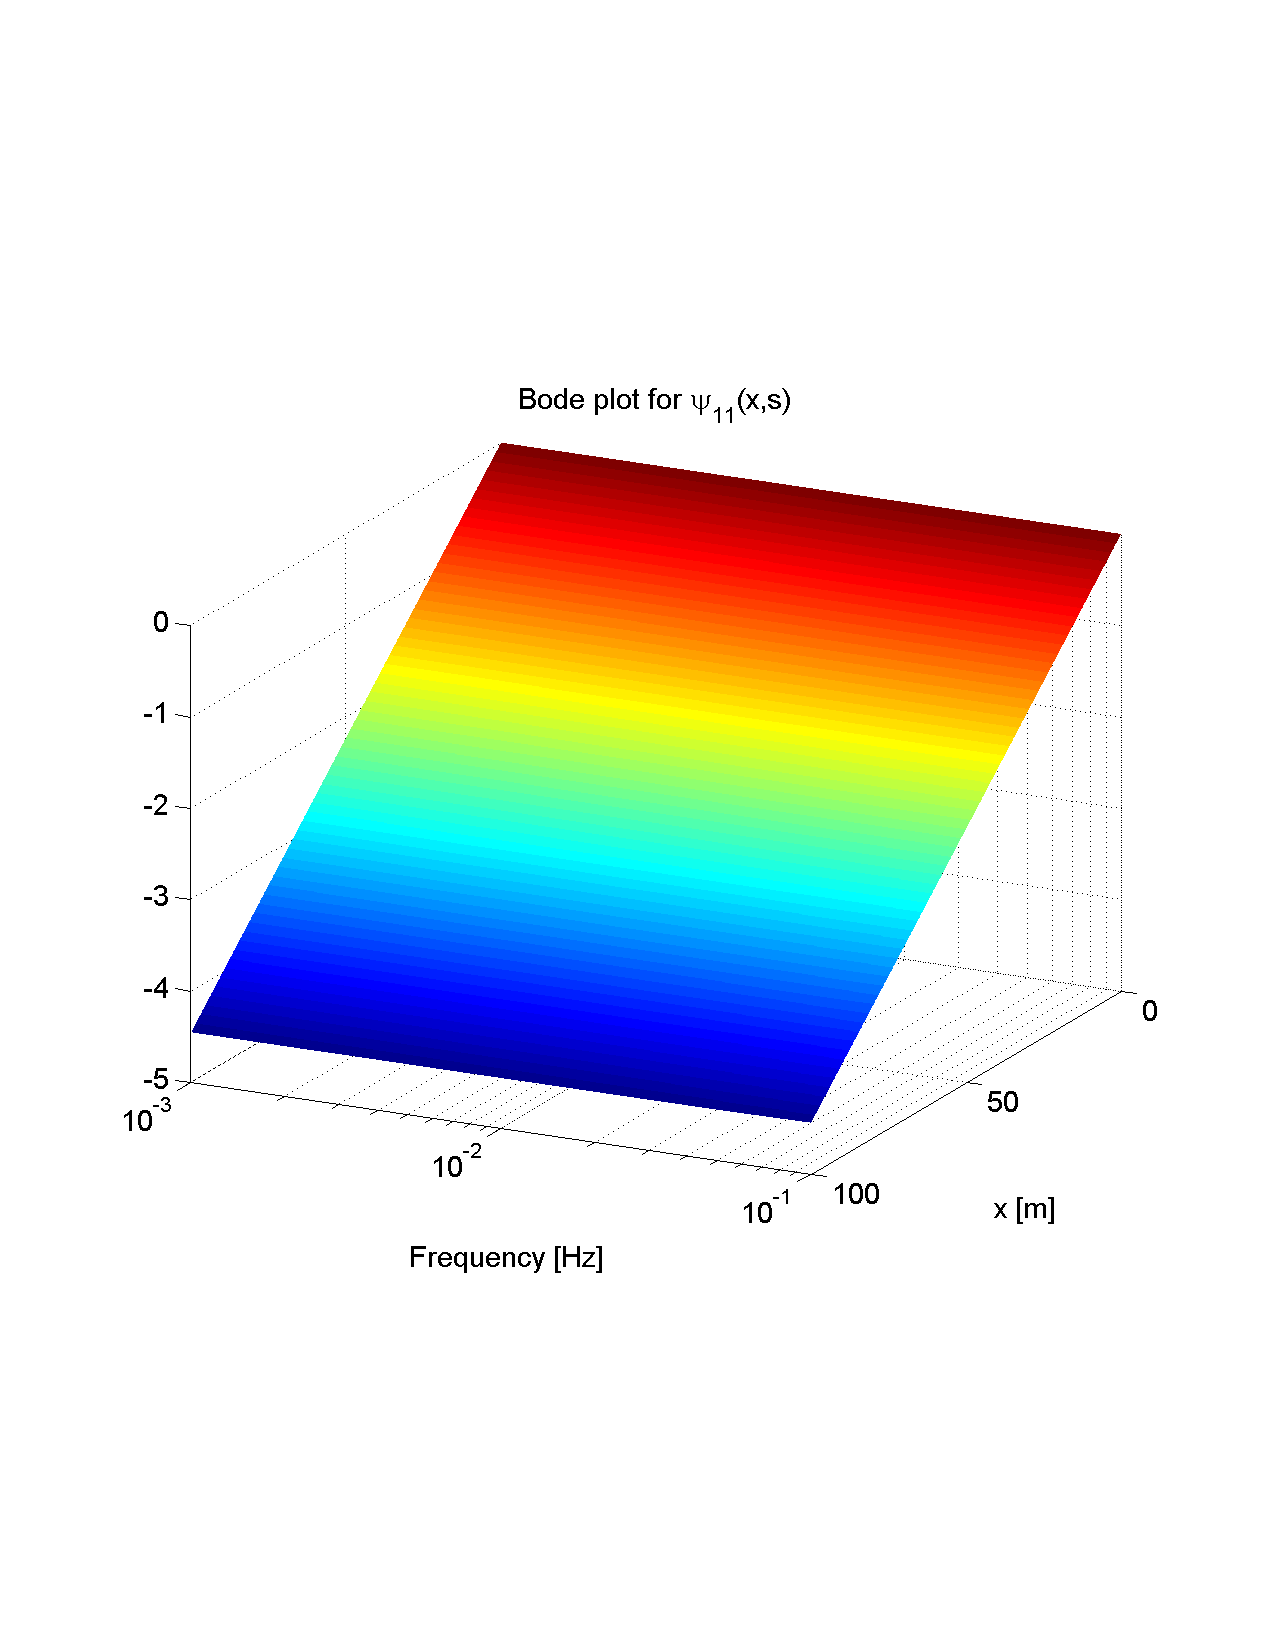
\includegraphics[trim = 0mm 60mm 0mm 60mm, width = 8cm]{distr11_-3to-1}
&
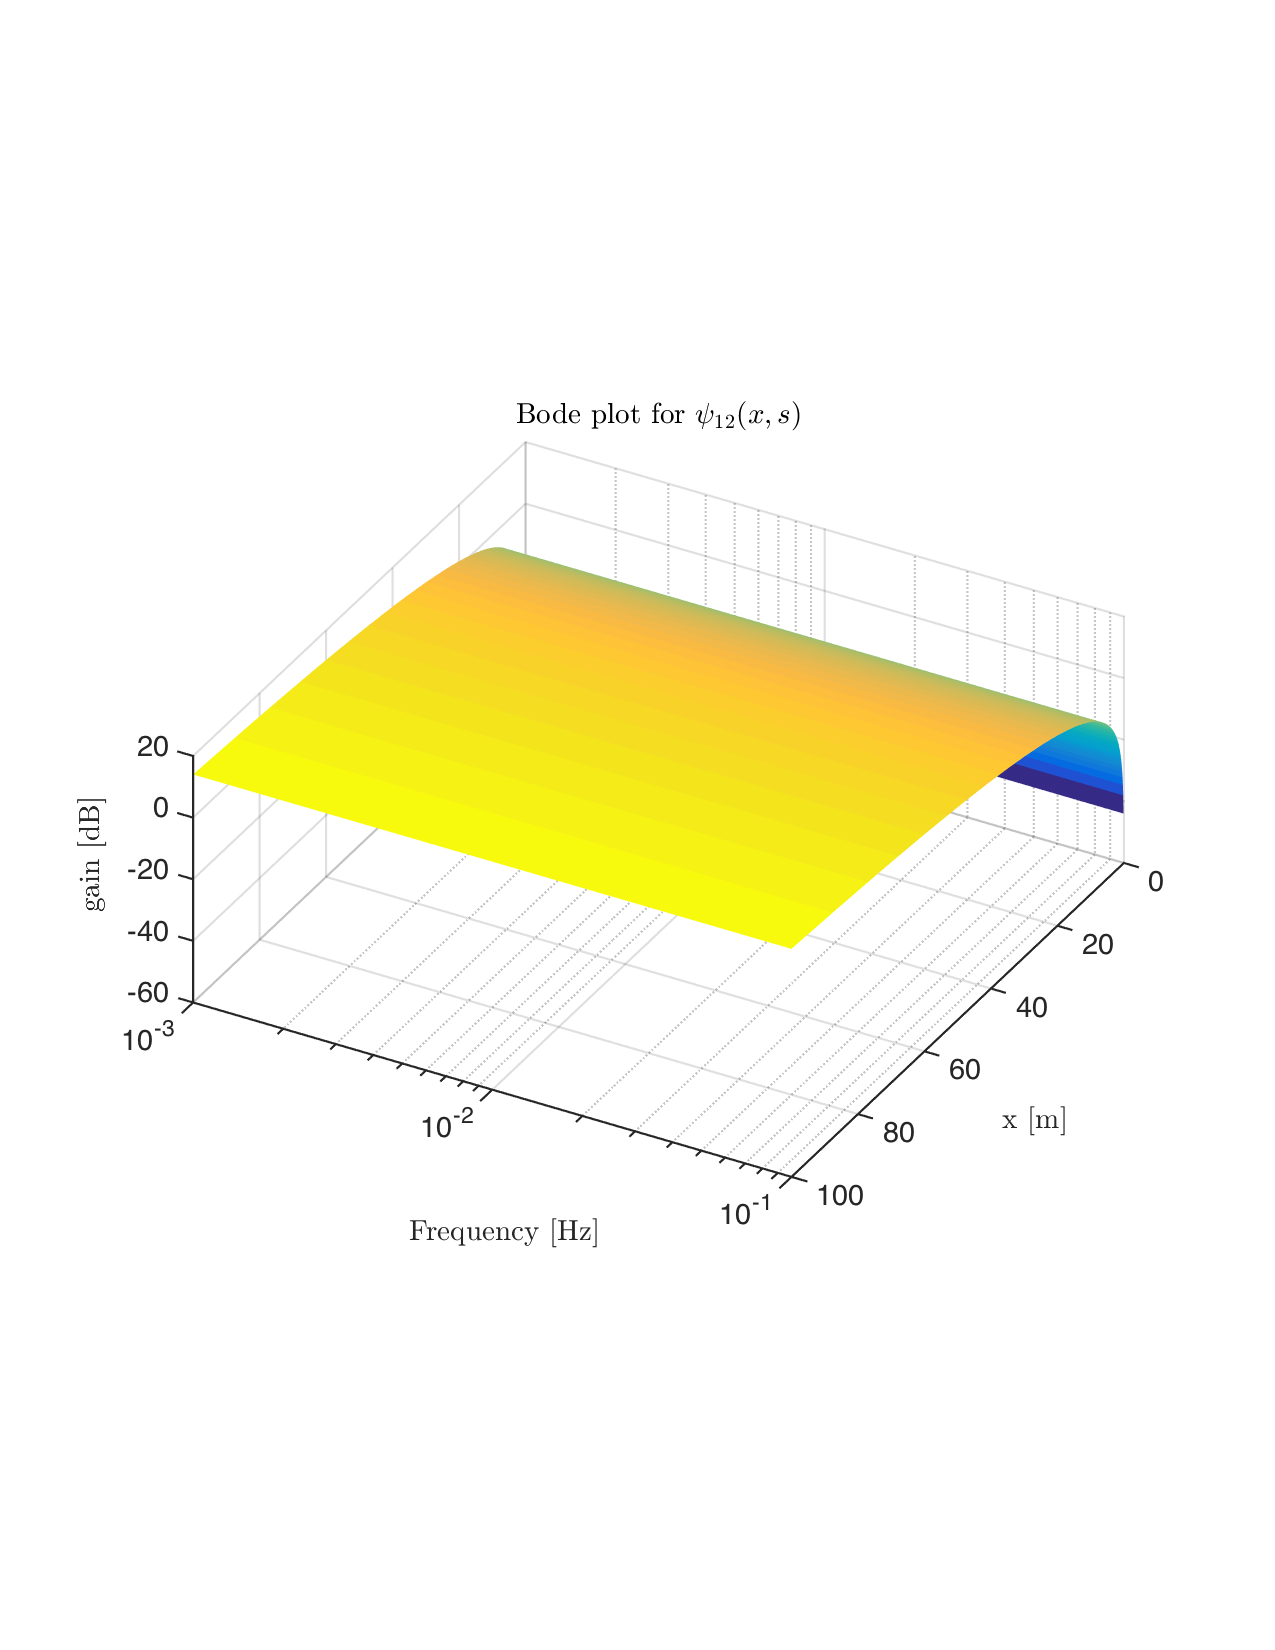
\includegraphics[trim = 0mm 60mm 0mm 60mm, width = 8cm]{distr12_-3to-1}
\tabularnewline
Spatial magnitude Bode plot for $\psi_{11}(x,s)$.
&
Spatial magnitude Bode plot for $\psi_{12}(x,s)$.
\tabularnewline
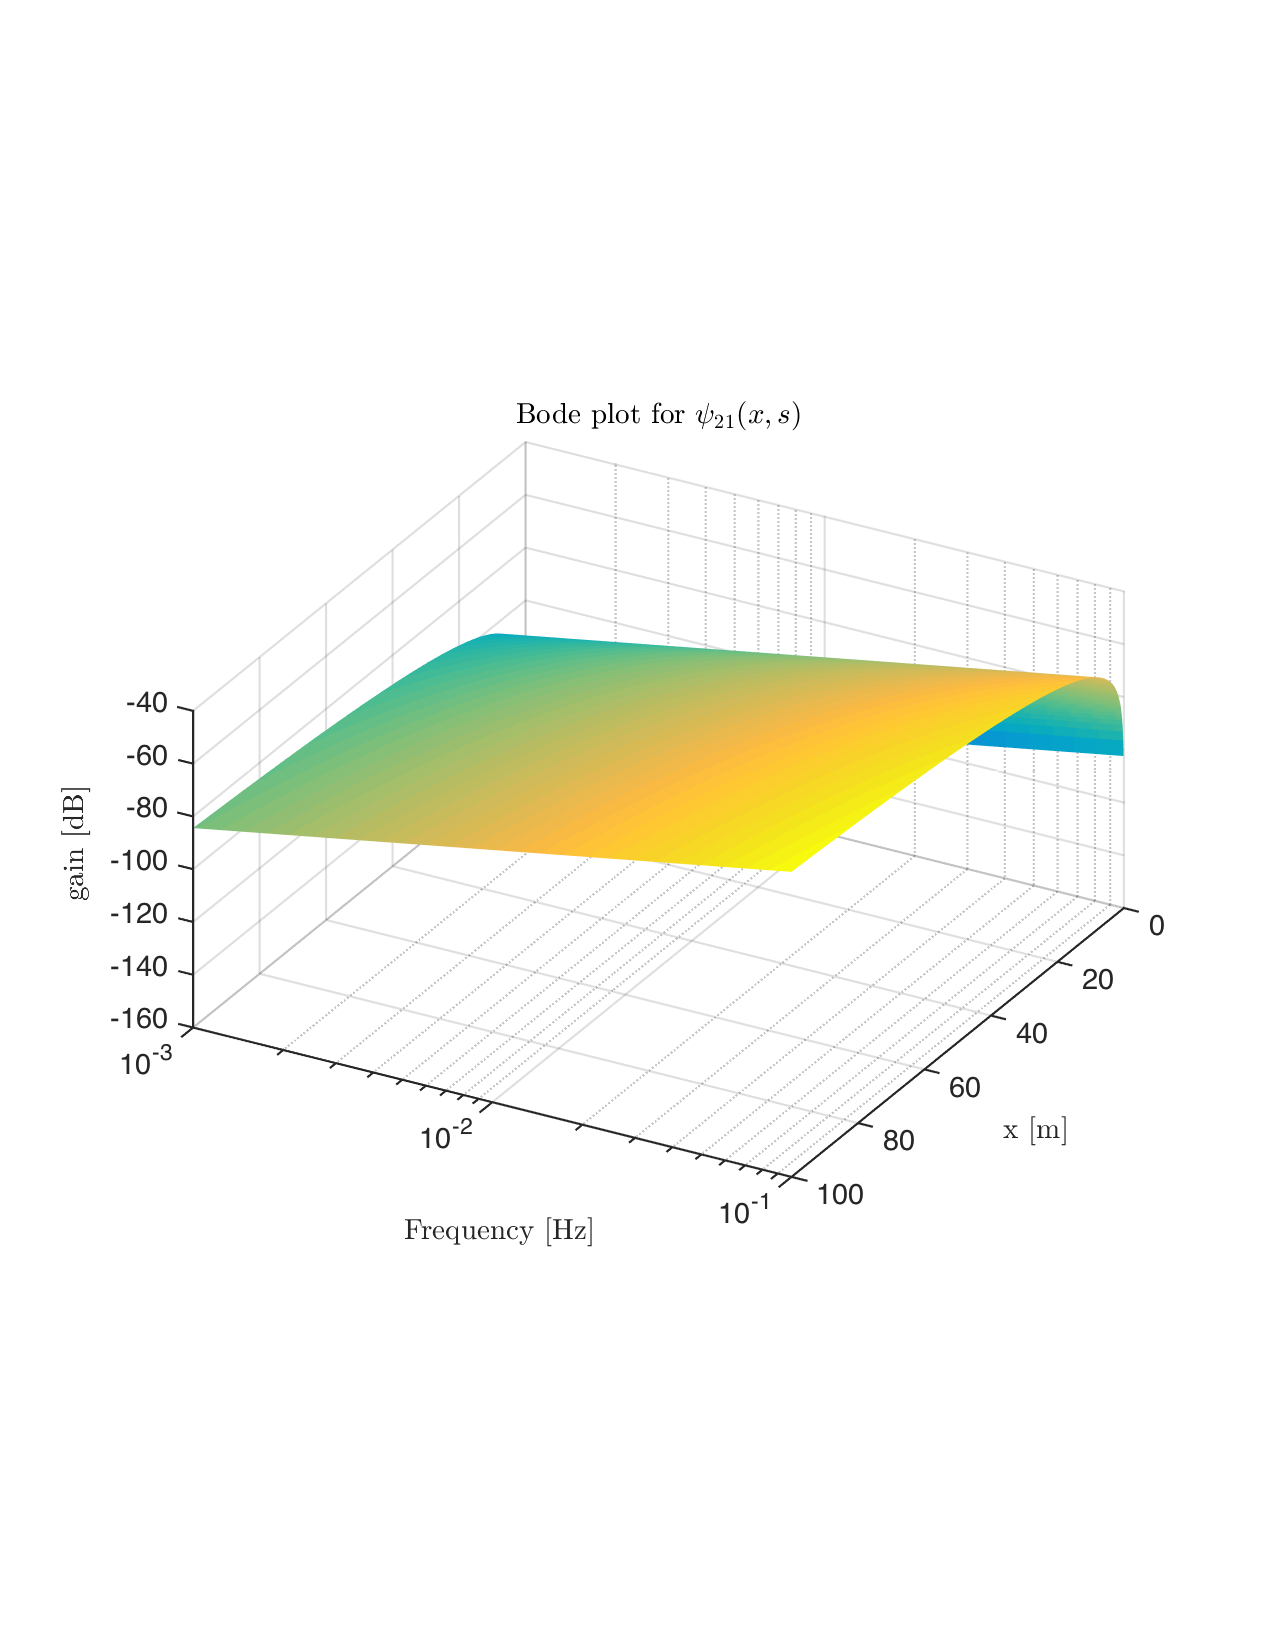
\includegraphics[trim = 0mm 60mm 0mm 60mm, width = 8cm]{distr21_-3to-1}
&
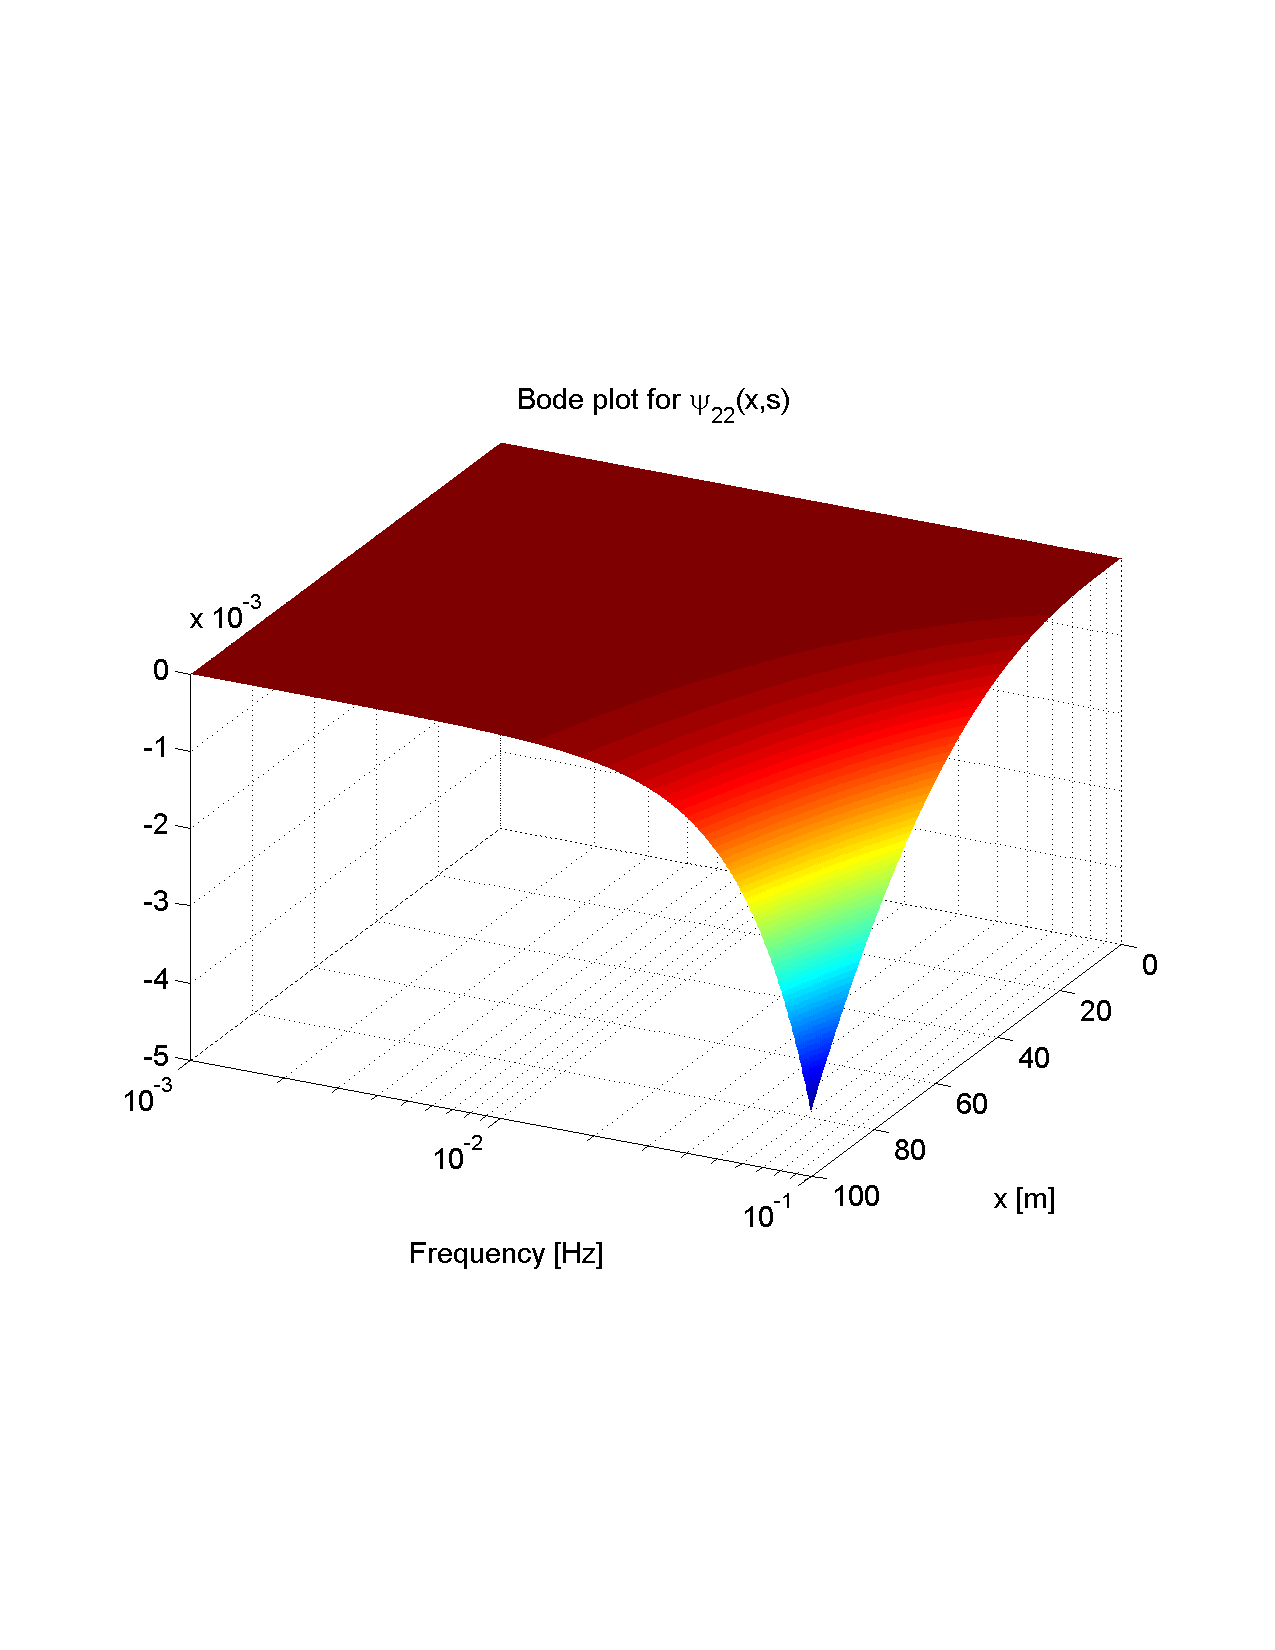
\includegraphics[trim = 0mm 60mm 0mm 60mm, width = 8cm]{distr22_-3to-1}
\tabularnewline
Spatial magnitude Bode plot for $\psi_{21}(x,s)$.
&
Spatial magnitude Bode plot for $\psi_{22}(x,s)$.
\tabularnewline
\end{tabular}
\caption{Spatial magnitude Bode plots for physical variables\label{Magn_spatial_physx}}
\end{figure}

\begin{figure}[H]
\centering
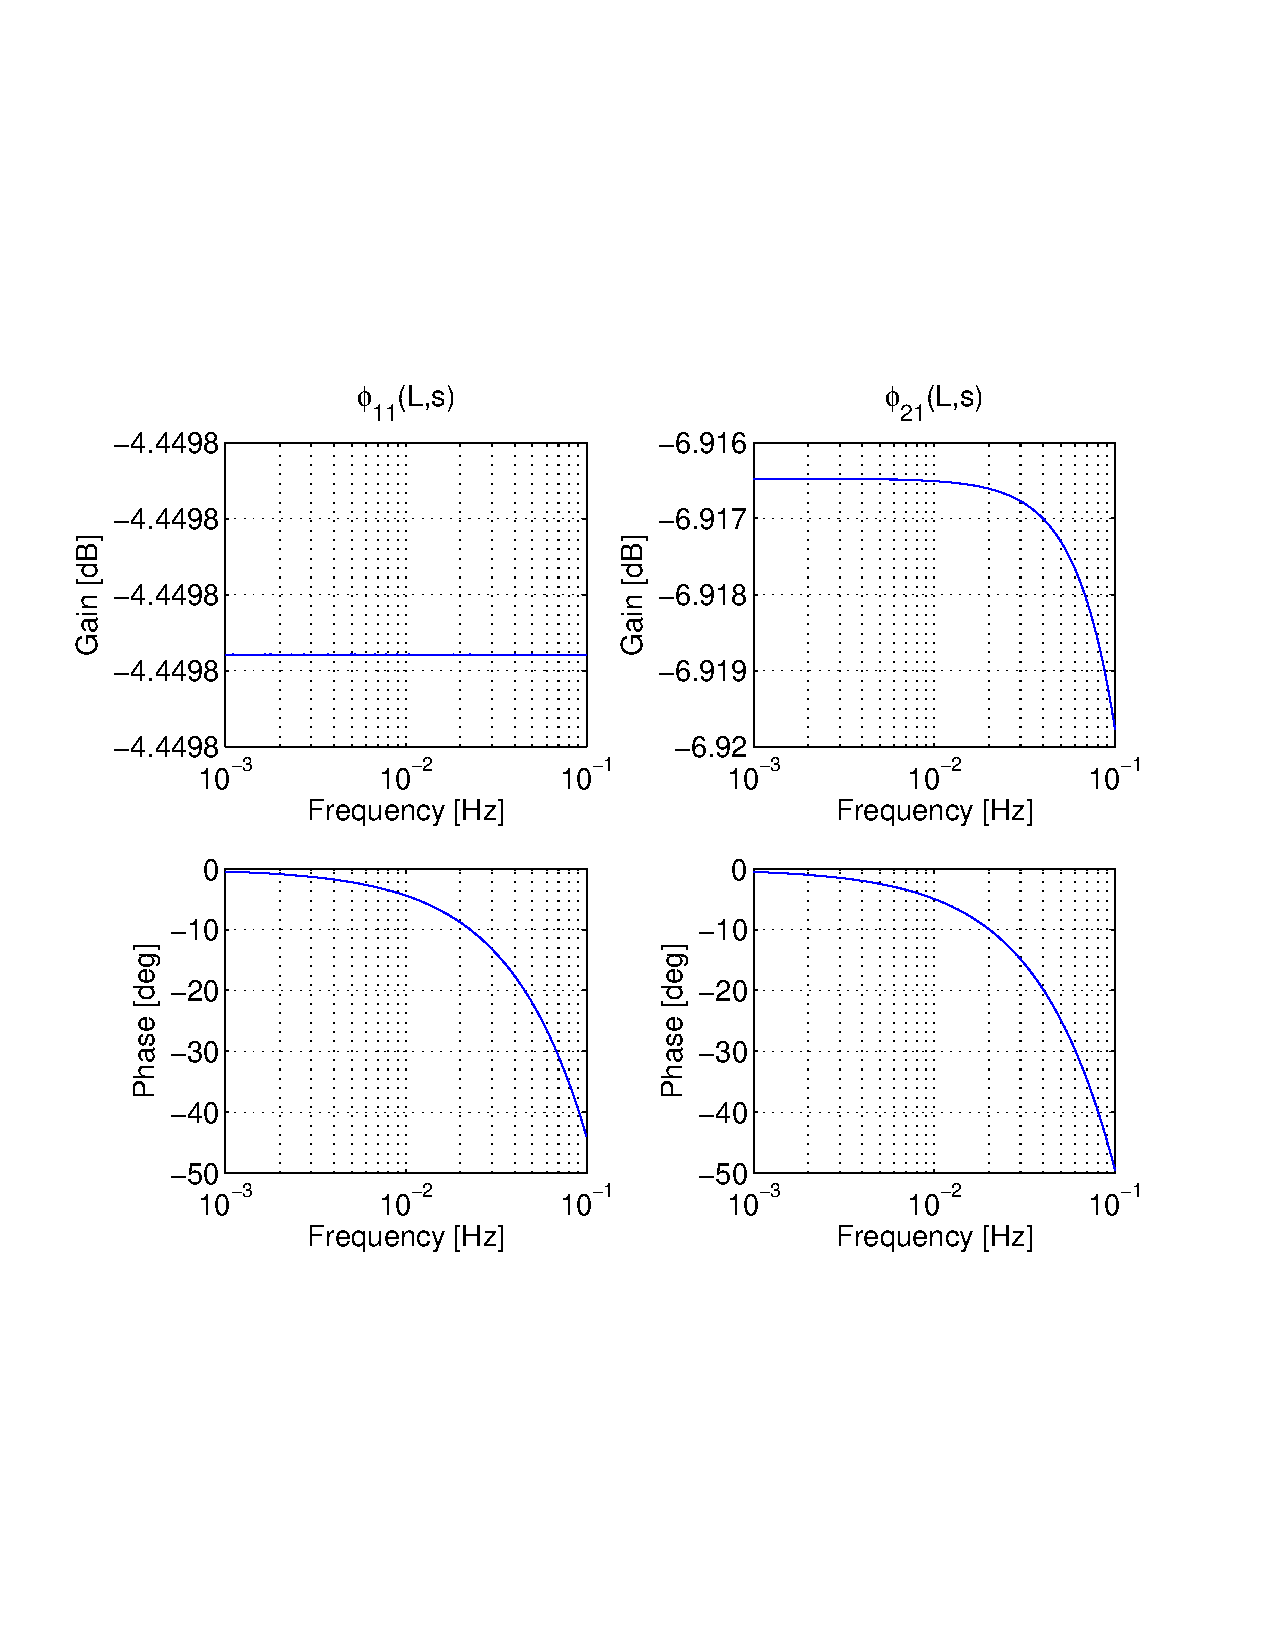
\includegraphics[trim = 0mm 60mm 0mm 60mm, width = 110mm]{diagIOfreeflow}
\caption{Magnitude and phase Bode plots for $\phi_{11}(L,s)$ and $\phi_{21}(L,s)$.\label{fig:Magn_phase_diag}}
\end{figure}

\begin{figure}
\centering
\begin{tabular}{cc}
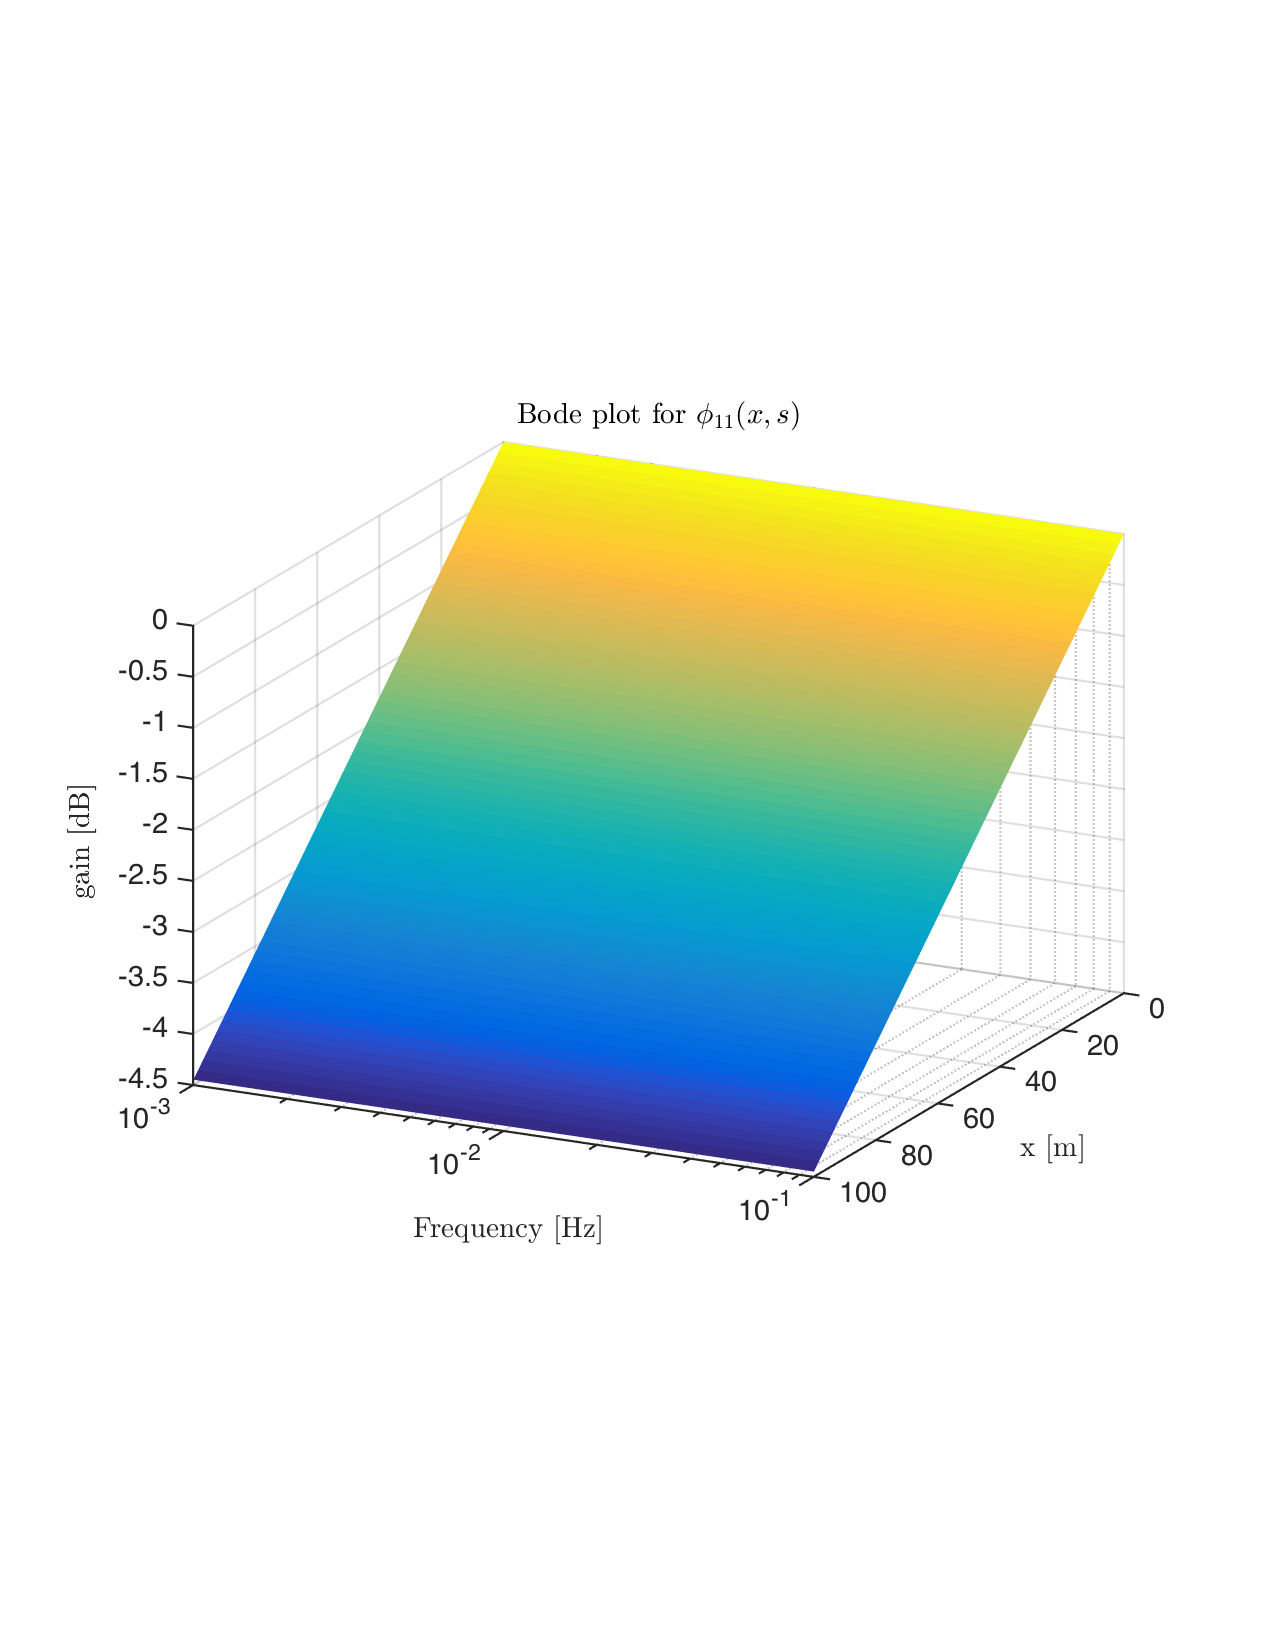
\includegraphics[trim = 0mm 60mm 0mm 60mm, width = 8cm]{diagdistr11freeflow}
&
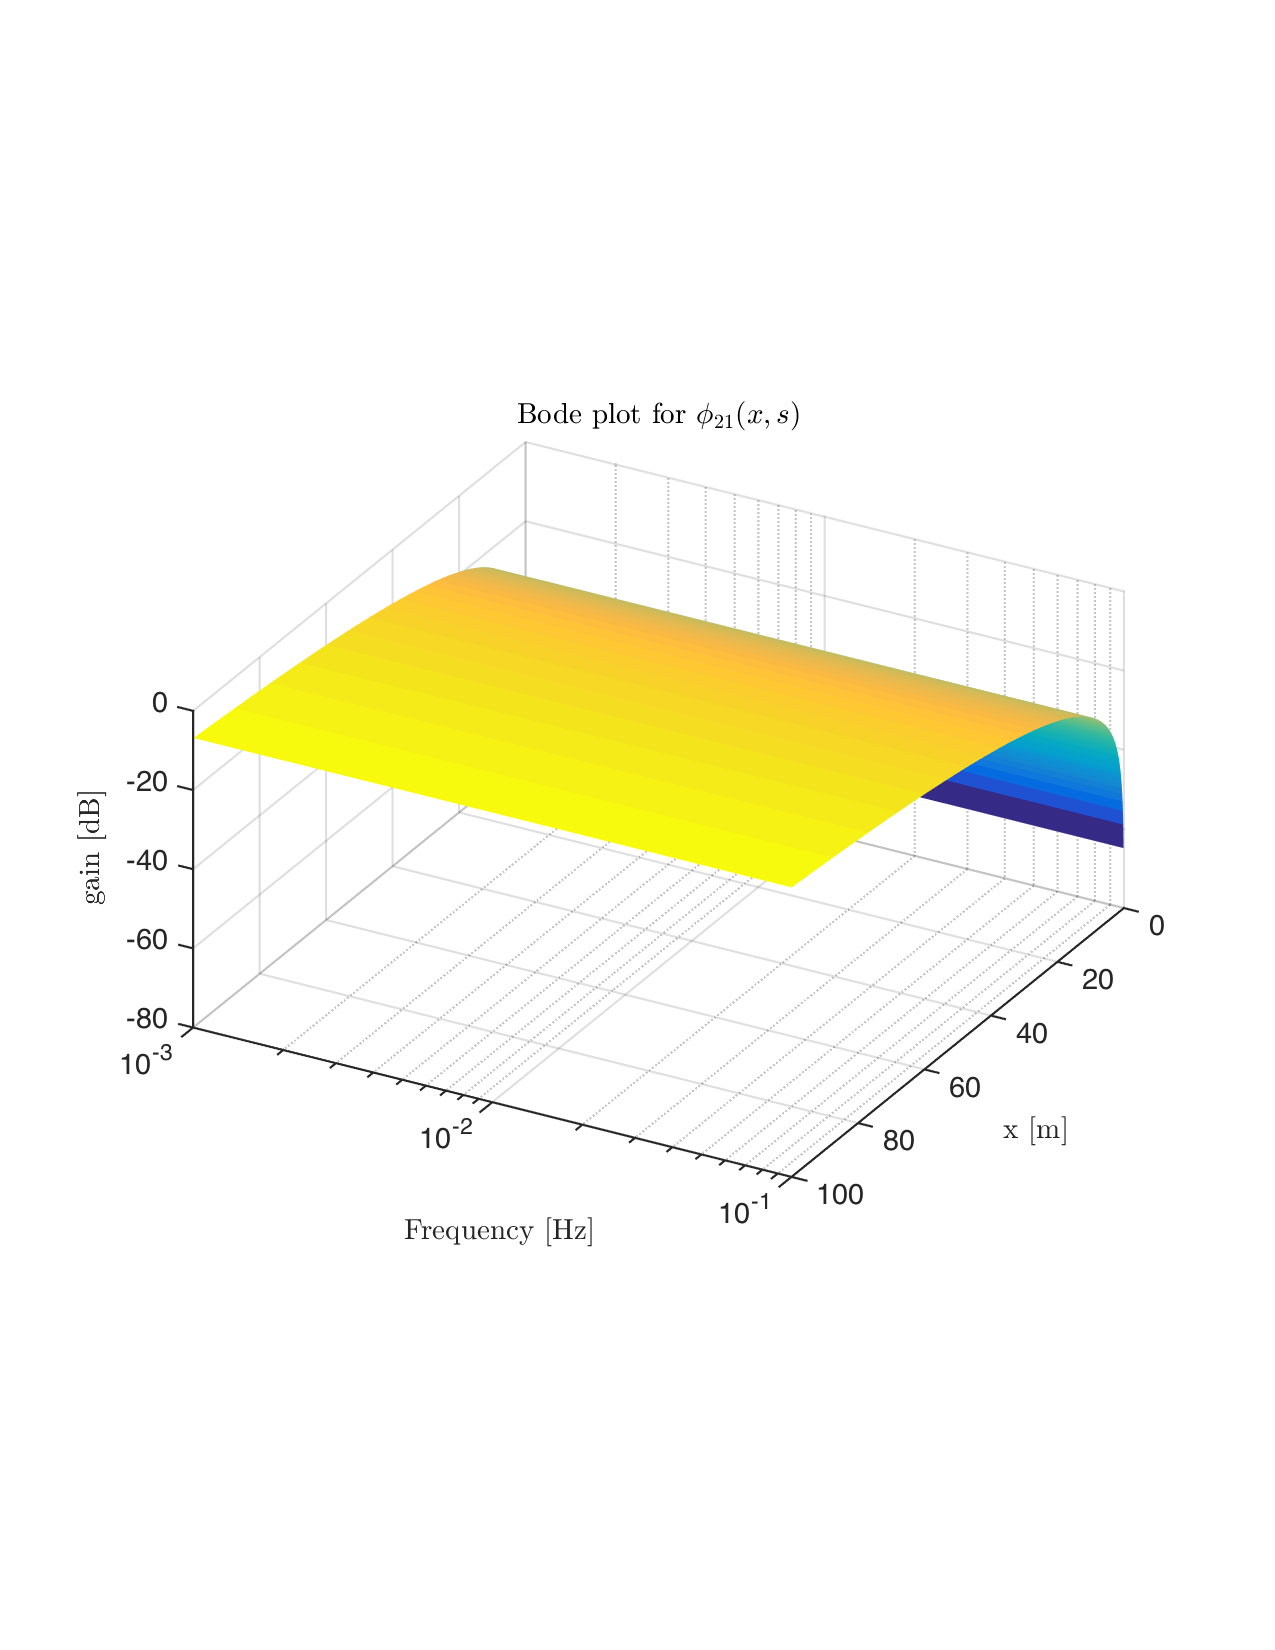
\includegraphics[trim = 0mm 60mm 0mm 60mm, width = 8cm]{diagdistr21freeflow}
\tabularnewline
Spatial magnitude Bode plot for $\phi_{21}(x,s)$.
&
Spatial magnitude Bode plot for $\phi_{22}(x,s)$.
\tabularnewline
\end{tabular}
\caption{Spatial magnitude Bode plots for Riemann invariants\label{Magn_spatial_diag}}
\end{figure}

\subsubsection{Step responses}
We analyze the behavior of the system given step inputs $v(0,t)=v_{step}H(t)$ and $q(0,t)=q_{step}H(t)$, where $H(\cdot)$ is the Heaviside function. The step responses are

\begin{align} 
v(x,t) &= v_{step}\left[e^{-\frac{x}{\lambda_1\tau}}\left(1 - e^{-a\left(t-\frac{x}{\lambda_1}\right)}\right)H\left(t-\frac{x}{\lambda_1}\right) + e^{-a\left(t-\frac{x}{\lambda_2}\right)}H\left(t-\frac{x}{\lambda_2}\right)\right] \notag \\
&\quad+ \dfrac{q_{step}}{\rho^* \tau}\left[- e^{-\frac{x}{\lambda_1\tau}}\left(1 - e^{-a\left(t-\frac{x}{\lambda_1}\right)}\right)H\left(t-\frac{x}{\lambda_1}\right) + \left(1 - e^{-a\left(t-\frac{x}{\lambda_2}\right)}\right)H\left(t-\frac{x}{\lambda_2}\right) \right] \\
q(x,t) &= v_{step}\rho^*\tau a\left[e^{-\frac{x}{\lambda_1\tau}}e^{-a\left(t-\frac{x}{\lambda_1}\right)}H\left(t-\frac{x}{\lambda_1}\right) - e^{-a\left(t-\frac{x}{\lambda_2}\right)}H\left(t-\frac{x}{\lambda_2}\right) \right] \notag \\
&\quad+ q_{step}\left[ e^{-\frac{x}{\lambda_1\tau}}e^{-a\left(t-\frac{x}{\lambda_1}\right)}H\left(t-\frac{x}{\lambda_1}\right) + \left(1 - e^{-a\left(t-\frac{x}{\lambda_2}\right)}\right)H\left(t-\frac{x}{\lambda_2}\right)\right]
\end{align}


\subsection{Congestion regime}
Consider now the system in the congestion regime. Here we have $\lambda_1 > 0, \lambda_2 < 0$, hence two boundary conditions are needed, one at the upstream boundary and one at the downstream boundary. A plot of the characteristics is shown in Figure \ref{fig:subcr}. \\

\begin{figure}[H] 
\centering
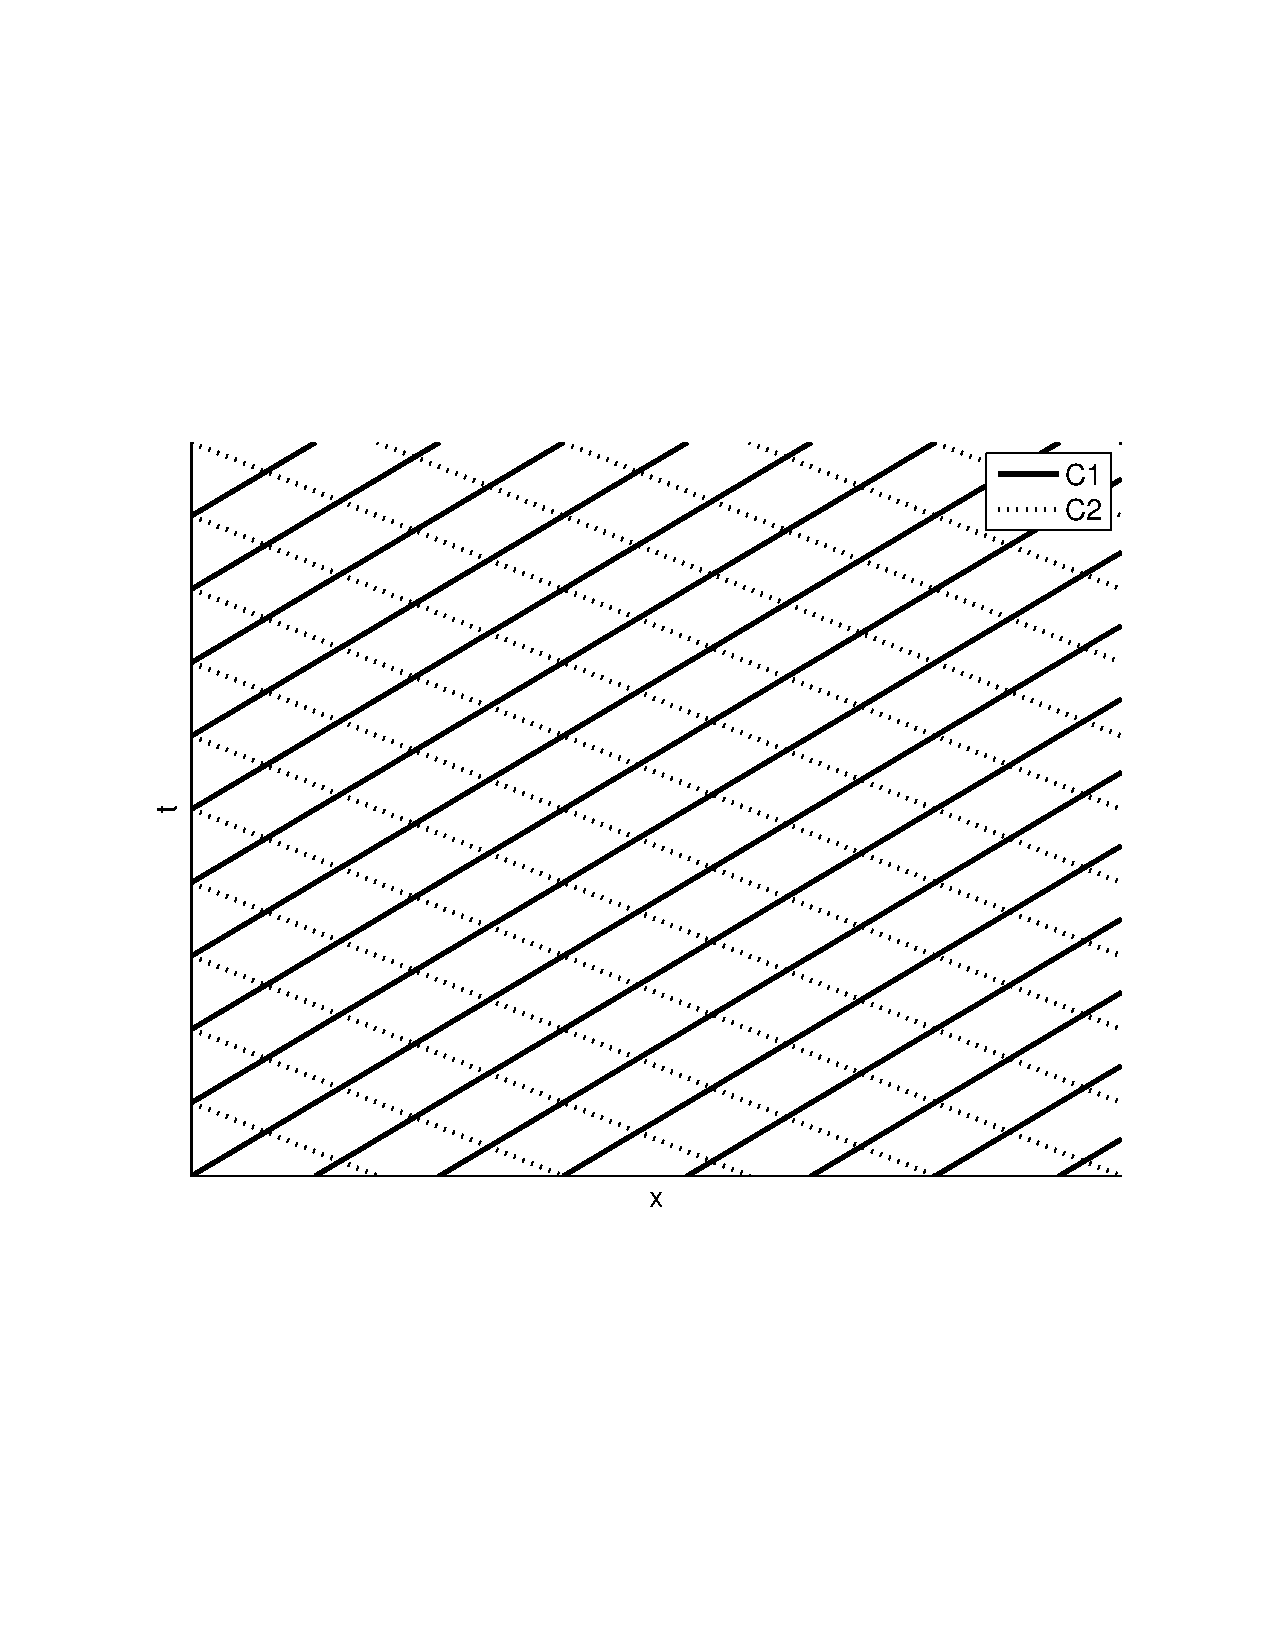
\includegraphics[trim= 0mm 75mm 0mm 70mm, width = 90mm]{subcr}
\caption{Illustration of the characteristics for supercritical flow, $\lambda_1 > 0, \lambda_2 < 0$.}
\label{fig:subcr}
\end{figure}


Using \eqref{TFRiemann} we can write 
\begin{equation}
\begin{pmatrix}
\hat{\xi_{1}}(x,s)\\
\hat{\xi_{2}}(x,s)
\end{pmatrix} = \underbrace{
\Phi(x,s) \begin{pmatrix}
1 & 0\\
-\frac{\phi_{21}\left(L,s\right)}{\phi_{22}\left(L,s\right)} & \frac{1}{\phi_{22}}
\end{pmatrix}}_\text{$\Gamma (x,s)$}
\begin{pmatrix}
\hat{\xi_{1}}\left(0,s\right)\\
\hat{\xi_{2}}\left(0,s\right)
\end{pmatrix}.
\end{equation}
with 
\begin{subequations}
\begin{align}
\gamma_{11}\left(x,s\right)&=e^{-\frac{x}{\lambda_{1}\tau}}e^{-\frac{sx}{\lambda_{1}}}, \\
\gamma_{12}\left(x,s\right)&=0, \\
\gamma_{21}\left(x,s\right)&=\alpha\frac{\lambda_{1}}{\lambda_{2}}\left(e^{-\frac{x}{\lambda_{1}\tau}}e^{-\frac{sx}{\lambda_{1}}}-e^{-\frac{L}{\lambda_{1}\tau}}e^{-\frac{s}{\lambda_{2}}\left(x-L\frac{\lambda_{1}-\lambda_{2}}{\lambda_{1}}\right)}\right)\frac{1}{s+\alpha}, \\
\gamma_{22}\left(x,s\right)&=e^{-\frac{s\left(x-L\right)}{\lambda_{2}}}.
\end{align}
\end{subequations}

\section{Numerical validation}

The ARZ equations provide a finer modeling of various phenomena affecting the dynamics of vehicular flow on a freeway. The spectral form of the linearized
model provides a simple framework for establishing control strategies for the system. Prior to
using such techniques, it is necessary to assess how realistic the
model is in its linearized form. This section compares the prediction of the model with actual flow
and velocity data gathered from the well-known NGSIM data set.


\subsection{Data source: NGSIM trajectories}

We use the NSGIM trajectory data set for a section of the US-101 highway. the set gathers trajectories of vehicles sampled with a 10 Hz frequency thanks to high precision cameras. The data is pre-processed so as to take only cars into account; 45 minutes are recorded on a 650-meter long section with five lanes. The lanes are taken into account when computing the lineic density of vehicles $\rho$.
The trajectories are represented in the $(t,x)$ domain
in Figure \ref{fig:NGSIM-trajectories}.
Only a subset of the spatial domain is used due to the presence of ramps, which breaks the homogeneity of the freeway. The viable domain is 200 meters long.

\begin{figure}[H]
\centering
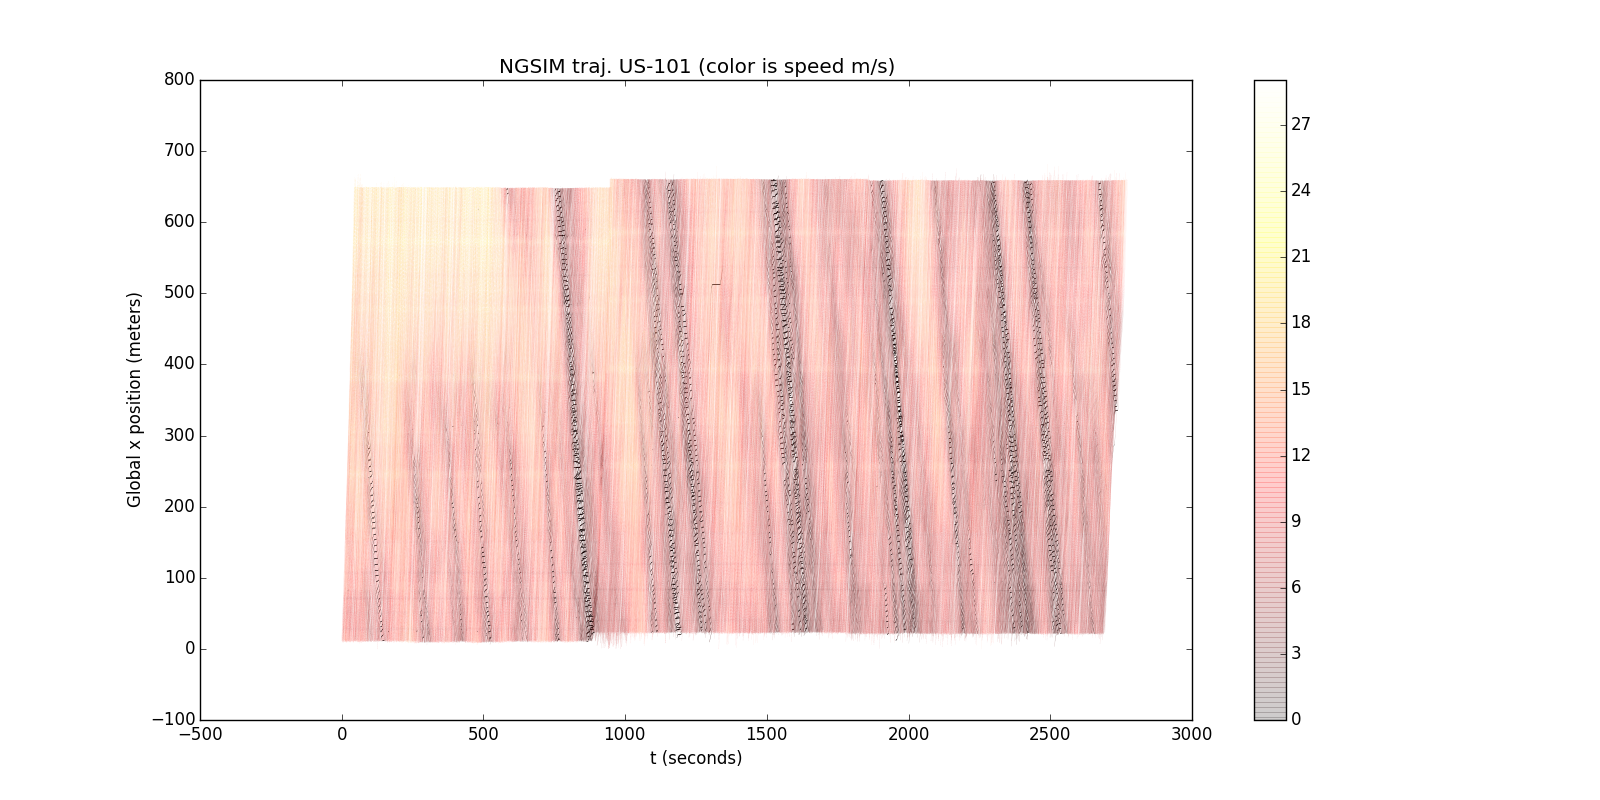
\includegraphics[width=12cm]{Numerics/US-101_all_traj_low_res}
\protect\caption{NGSIM trajectories. Color represents the measured speed of each
car in m/s.}
\label{fig:NGSIM-trajectories}
\end{figure}



\subsection{Reconstructing $(v,q)$ maps from NGSIM trajectories}

The NGSIM data set does not directly provide the values $v(t,x)$
and $q(t,x)$ in the resolution domain $\left[0,T\right]\times\left[0,L\right]$.
In order to obtain macroscopic quantities out of the microscopic measurements,
we divide the space-time grid
into small bins $\left(\left[i\Delta t,\, \left(i+1\right)\Delta t\right]\times\left[j\Delta x, \, (j+1)\Delta x\right]\right)_{i\in\left\{ 1\ldots n_{t}\right\} ,j\in\left\{ 1\ldots n_{x}\right\} }$, where $n_t$ and $n_x$ are the number of bins in time and space, respectively. This operation consists of gathering corresponding data points into bins, then estimating the quantities of interest in each bin. 

\noindent \textbf{Binning formulae}

The size of each bin is $\Delta t\times\Delta x$. Within each bucket, a finite number of traces, or footprints of a vehicle along its trajectory, are available, and $\rho$, $v$, and $q$ are assumed to be constant. We present several formulae to map a set of traces to speed, flow, and density over the space-time grid. 

\textit{Binning formula for $v$}: Since the speed is assumed to be constant in each bin, a straightforward estimate for the speed is the empirical average. Let $\widehat{v}_{i,j}$ be the estimator for the speed in bin $(i,j)$:

\begin{equation}
\widehat{v}_{i,j}=\mean_{\trc \in \bin_{i,j}}(v(\trc))
\end{equation}

\textit{Binning formula for $\rho$}: Consider a bin with index $(i,j)$. By definition, 
\begin{equation}
\rho_{i,j}=\frac{1}{n_{\lns}\Delta x\Delta t}\iint_{\left(t,x\right)\in [i\Delta t, \,(i+1)\Delta t] \times [j\Delta x,\,(j+1)\Delta t]}\rho(x,t) \text{d}x \text{d}t.
\end{equation}

The position of each vehicle is recorded every 0.1 second. We count the number of traces in a given bin and normalize it by the sampling rate. The contribution of a given vehicle to the density of a bin is proportional to the
number of traces it has left in the bin. If the speed is assumed to be locally constant, this contribution is proportional to the time this vehicle spends in the bin and is consistent with the conservation of the total number of vehicles across all bins.

\begin{equation}
\widehat{\rho}_{i,j}=\frac{1}{n_{\lns} \Delta x \Delta t \: \text{sampling rate}}\card ( \{ \trc \mid \trc \in \bin \} ),
\end{equation}
where $\card (\cdot)$ gives the number of elements in a set, i.e., its cardinal.

\textit{Binning formula for $q$}:

By definition, $q\left(x,t\right)=\rho\left(x,t\right)v\left(x,t\right)$, so a logical first estimate for $q$ in bin $(i,j)$ is 
\begin{equation}
\widehat{q}_{i,j}=\widehat{v}_{i,j}\widehat{\rho}_{i,j}.
\end{equation}

We can also approximate the flux going through a given bucket $\left[i\:\Delta t,\:\left(i+1\right)\:\Delta t\right]\times\left[j\:\Delta x,\:\left(j+1\right)\:\Delta t\right]$
by the number of cars crossing the $x$ coordinate $\left(j+1\right)\Delta x$
between times $i\:\Delta t$ and $\left(i+1\right)\Delta t$ normalized
by the duration $\Delta t$.

If a given vehicle with identification number id crosses $\left(j+1\right)\Delta x$
between time $i\Delta t$ and time $\left(i+1\right)\Delta t$,
then id is present in bins $\left[i\Delta t,\,\left(i+1\right)\Delta t\right]\times\left[j\Delta x,\,\left(j+1\right)\Delta t\right]$
and $\left[i\Delta t,\,\left(i+1\right)\Delta t\right]\times\left[\left(j+1\right)\Delta x,\,\left(j+2\right)\Delta t\right]$.
Therefore, $\card\left(\left\{ \text{id}\left(\trc \right)\mid \trc \in \bin_{i,j}\right\} \cap\left\{ \text{id} \left(\trc\right)\mid \trc\in \bin_{i,j+1}\right\} \right)$
is the number of vehicles that have crossed the coordinate $\left(j+1\right)\Delta x$
in that interval of time. This gives another estimator of the flux
based on counting cars in a straightforward way: 
\[
\widehat{q}_{i,j}^{\cnt}=\frac{1}{n_{\lns}\Delta t}\: \card\left(\left\{ \text{id} \left(\trc\right)\mid \trc \in \bin_{i,j}\right\} \cap\left\{ id\left( \trc \right)\mid \trc\in \bin_{i,j+1}\right\} \right)
\]



\subsubsection{Choosing the number of bins}

The discretization grid is $\left\{ \left[i\:\Delta t,\:\left(i+1\right)\:\Delta t\right]\times\left[j\:\Delta x,\:\left(j+1\right)\:\Delta t\right]\mid\left(i,j\right)\in\left\{ 1\ldots N\right\} \times\left\{ 1\ldots N\right\} \right\} $.
As the estimation formulae above rely on averaging, having a comfortable
number of points in each bin provides more stable estimates. It is
worth mentioning that usual Central Limit theorem based reasoning
for convergence of such estimates is flawed as several samples may
correspond to the same vehicle or interacting vehicles, therefore
violating the independence assumption of the theorem. Proving the
convergence of the estimates above lies clearly beyond the scope of
this article and therefore, as a rule of thumb we choose a setup that
guarantees that most bins will host more than $100$ traces. This
is achieved with a $80\times80$ grid where the $10^{th}$ percentile
of the number of traces in a given bin is $170$. Such a grid also
yields a $10^{th}$ percentile of $56$ distinct vehicles per bin.
The histograms of number of traces and vehicle per bin are represented
on Figure \ref{fig:Grid control}.

\begin{figure}[H]
\centering
\begin{tabular}{cc}
\includegraphics[width=8cm]{\string"/Numerics/Discretisation grid/traces_80_80\string".png} & \includegraphics[width=8cm]{\string"/Numerics/Discretisation grid/ids_80_80\string".png}\tabularnewline
Histogram of number of traces per bin & Histogram of number of distinct vehicles per bin \tabularnewline
\end{tabular}
\caption{Choice motivation for a $80\times 80$ bin based discretization
grid for the NGSIM data}
\label{fig:Grid control}
\end{figure}



\subsubsection{Sanity check for the estimators}

This article does not provide any theoretical proof of the convergence
of the binned estimators for $\left(v,\rho,q\right)$ presented above.
It is nonetheless possible to check practically that the procedure
is coherent. Two estimators are provided for $q$ that use radically
different techniques. The first one relies on the average measured
speed and the number of traces in a bin. The other one on counting
vehicles transiting from a cell to another. Verifying that they both
give similar results for a given bucket will therefore confirm that
these estimators for $q$ are trustworthy. It will also certify that
the estimation technique for $\rho$ is valid. As one can observe
on Figure \ref{fig:Sanity-check}, the scatter plot of $\widehat{q}_{i,j}^{count}$
is plotted against $\widehat{q}_{i,j}$ coincides almost perfectly
with the line $y=x$ therefore validating the overall binning and
estimation procedure.

\begin{figure}[H]
\centering
\includegraphics[width=8cm]{\string"/Numerics/Sanity check/80_80_q_q_count\string".png}
\protect\caption{Sanity check for the estimation procedure. $\widehat{q}_{i,j}^{count}$
is plotted against $\widehat{q}_{i,j}$ across the grid of bins.
\label{fig:Sanity-check}}
\end{figure}



\subsection{Estimated values for $\left(v,q\right)$}

In order to check how well the linearized ARZ model fits actual data,
one choses a bounded domain and compares the theoretical solution
given by the second order model and the data observed. Here we focus
one the values of $v$ and $q$ as they correspond to the setup that
is the most worth studying. It is also the most directly practical
for control. Now that estimates of the actual values of $v$ and $q$
have been designed, they will be used to compute fundamental diagrams
and mapped on the $\left[0,T\right]\times\left[0,L\right]$ domain.
Fundamental diagrams will then yield estimates of the eigen values
$\lambda_{1}$ and $\lambda_{2}$ that are crucial in this study.
Finally, predicted values of $v$ and $q$ will be compared to their
measured counterparts which will allow the computation of a fit error.
Based on the estimation of this error for different values of the
parameter $\tau$, the value offering the best fit will be used
as an estimate. Plotting maps of both the predicted values and the
observed one will also highlight the phenomena the linearized model
accounts for and those it cannot characterize.


\subsubsection{Maps}

Once the values $\widehat{v}_{i,j}$, $\widehat{\rho}_{i,j}$, $\widehat{q}_{i,j}$,
$\widehat{q}_{i,j}^{count}$ have been computed they can be plotted
on the discretization grid (see Figure \ref{fig:Estimated-values}).
As $\widehat{q}$ and $\widehat{q}^{count}$ give extremely similar
results, $\widehat{q}^{count}$ will be used as the estimator of $q$
from now on.
Damped oscillations
and smoothly decaying values along characteristic lines are the main characteristic the practical implementation of the model should feature.

\begin{figure}[H]
\centering
\begin{tabular}{cc}
\includegraphics[width=8cm]{\string"/Numerics/Maps data/80_80_v_map\string".png} & \includegraphics[width=8cm]{\string"/Numerics/Maps data/80_80_rho_map\string".png}\tabularnewline
\includegraphics[width=8cm]{\string"/Numerics/Maps data/80_80_q_map\string".png} & \includegraphics[width=8cm]{\string"/Numerics/Maps data/80_80_q_count_map\string".png}\tabularnewline
\end{tabular}
\protect\caption{Estimated values for $\left(v,q,\rho\right)$. Top left: $\widehat{v}_{i,j}$.
Top right: $\widehat{\rho}_{i,j}$. Bottom left: $\widehat{q}_{i,j}$.
Bottom right: $\widehat{q}_{i,j}^{count}$ .\label{fig:Estimated-values}}
\end{figure}



\subsubsection{Fundamental diagrams}

From the values that have been estimated it is very straightforward
to compute fundamental diagrams as on Figure \ref{fig:Empirical-fundamental-diagrams}.
One of the potential flaws of studying these fundamental diagrams
and using them to calibrate the model's parameters as we do below
could come from the fact that the data set is small. Even though many
points are collected, they only give information about cars traveling
in a small region of time and space. Therefore it is certain that
our measurements are highly correlated. This seems
to be confirmed by the fact that the fundamental diagrams below only
correspond to the congested regime. Most of the points are concentrated
about the same region. This is not enough to guarantee that the estimated
quantities are reliable. However, NGSIM is to this day one of the
most comprehensive data sets of vehicle behavior on a freeway. It
is therefore one of the best ways one has to validate that a traffic
model is realistic. The fact that most points lie in the same region
is also a sign that the linearization hypothesis is reasonable
in that context. Observed deviations from the equilibrium are indeed
generally small. (The equilibrium, i.e. the linearization point, is estimated
below).

\begin{figure}[H]
\centering
\begin{tabular}{ccc}
\includegraphics[width=5cm]{\string"/Numerics/Maps data/80_80_fundamental_diagram_rho_q_count\string".png} & \includegraphics[width=5cm]{\string"/Numerics/Maps data/80_80_fundamental_diagram_v_q_count\string".png} & \includegraphics[width=5cm]{\string"/Numerics/Maps data/80_80_fundamental_diagram_v_q_count\string".png}\tabularnewline
\end{tabular}
\protect\caption{Empirical fundamental diagrams. Left: $\left(\widehat{\rho},\widehat{q}^{count}\right)$.
Middle: $\left(\widehat{v},\widehat{q}^{count}\right)$. Right: $\left(\widehat{\rho},\widehat{v}\right)$.
\label{fig:Empirical-fundamental-diagrams}}
\end{figure}



\subsubsection{Calibration of $\lambda_{1}$ and $\lambda_{2}$, linearization point}

$\lambda_{1}=v^{*}$ and $\lambda_{2}=Q'\left(v^{*}\right)$ therefore
the calibration of $\lambda_{1}$ consists in finding a value of $v$
around which the fundamental diagram $\left(v,q\right)$ will be linearized.
$\lambda_{2}$ will consist in the estimated slope of the fundamental
diagram. $\lambda_{2}$ is estimated with a standard Ordinary Least
Squares method. The data set above only corresponds to the congested
regime and the fundamental diagram is almost affine.\\
\\
The method used here is therefore quite straightforward. The estimator
for $v^{*}$ is chosen as the empirical mean of $\widehat{v}_{i,j}$:
$\widehat{\lambda}_{1}=\widehat{v}^{*}$. A linear model is fitted:
$\widehat{q}^{count}=b_{1}\widehat{v}+b_{0}+\varepsilon$ (where $\varepsilon$
represents the noise in the model that would ideally be centered,
homoschedastic and uncorrelated but is not practically) and the estimator
for $\lambda_{2}$ is then $\widehat{\lambda}_{2}=\widehat{b}_{1}$.
$q^{*}$ is estimated by the empirical average of $\widehat{q}^{count}$
and $\rho^{*}$ by the ratio of the estimates for $q^{*}$ and $v^{*}$.
Provided each estimator is convergent, the continuity of the functional
$\left(x,y\right)\rightarrow\frac{x}{y}$ on its domain guarantees
the convergence of the estimator for $\rho^{*}$. The empirical results are presented on Figure \ref{fig:Calibration-of-eigen-values}.
The determination coefficient is mediocre, it could be improved
by filtering out outliers and more generally by gathering more data.
Improving the quality of the estimation will be the subject of further
work on that matter. Significance tests for the coefficients of the
linear model are not presented. The assumptions they rely on about
the linear depency between $\widehat{q}$ and $\widehat{v}$ are clearly
not respected here as the noise is auto-correlated. Further
work needs to turn this rather heuristic method for estimating parameters
into a fully justified statistical procedure. This article focuses
is qualitatively assessing what phenomena can be accounted for by
the linearized second order model.

\begin{figure}[H]
\centering
\begin{tabular}{cccccc}
\multicolumn{6}{c}{\includegraphics[width=8cm]{\string"/Numerics/Calibration of eigen values/Fundamental diagram fitting n = 80\string".png}}\tabularnewline
$\widehat{\lambda}_{1}=8.96$ & $\widehat{\lambda}_{2}=-4.37$ & $\widehat{\rho}^{*}=0.049$ & $\widehat{v}^{*}=8.96$ & $\widehat{q}^{*}=0.44$ & $r^{2}=0.48$\tabularnewline
\end{tabular}
\protect\caption{Calibration of $\lambda_{1}$ and $\lambda_{2}$. The figure shows
the average point used to compute $\widehat{v}^{*}$ and $\widehat{q}^{*}$.
The affine model used to estimate $\lambda_{2}$ is also plotted.\label{fig:Calibration-of-eigen-values}}
\end{figure}



\subsection{Simulated values for $\left(v,q,\rho\right)$}

The data above shows that only the congested regime is to be modeled
for the NGSIM data. Therefore the theory developed for the $\lambda_{2}<0$
will be put to use here.


\subsubsection{Fourier decomposition of input for a linear PDE}

The Partial Differential Equation under scrutiny here is linearized.
Therefore, decomposing boundary conditions into a sum and then adding
the predicted values inside the domain $\left[0,T\right]\times\left[0,L\right]$
will give the exact solution. The spectral domain analysis presented
above is very useful to that end and will be leveraged thanks to Fourier
analysis. Fourier transform is a linear operator that is practically
implemented thanks to the Fast Fourier Transform. A real signal $\left\{ f\left(t\right)\mid t\in\left[0,T\right]\right\} $
on one of the boundaries $\left\{ \left(x=0,t\right)\mid t\in\left[0,T\right]\right\} $
or $\left\{ \left(x=L,t\right)\mid t\in\left[0,T\right]\right\} $
is transformed into a periodic signal by infinite duplication and
then turned into a Fourier series $\left\{ t\rightarrow\mu+\sum_{k=1}^{n}\beta_{k}\cdot cos\left(k\cdot wt+\phi_{k}\right)H\mid t\in\left[0,T\right]\right\} $.
This process is known to be convergent with an infinite sum for any
square integrable function. It is practically extremely accurate in
our case even though the FFT only relies on a finite number of Fourier
coefficients. For both upstream and downstream boundary conditions,
eye inspection cannot distinguish the original signal from its Fourier
series decomposition. In Appendix \ref{sub:Generic-computations}
the generic way of computing the solution of the PDE inside the inner
domain is presented. The process is quite straightforward although
the necessary computations are somewhat cumbersome.


\subsubsection{Simulated maps}

Prior to using Fourier decomposed signals and elementary solutions,
it is necessary to convert the data into the diagonalized basis. First
of all, the difference with respect to the equilibrium is computed
for each bin: $\widehat{\widetilde{v}}_{i,j}=\widehat{v}_{i,j}-\widehat{v}^{*}$,
$\widehat{\widetilde{q}}_{i,j}=\widehat{q}_{i,j}-\widehat{q}^{*}$.
Once $\lambda_{1}$ and $\lambda_{2}$ have been estimated, estimates
for $\xi_{1}$ and $\xi_{2}$ are computed thanks to the following
equations: $\widehat{\xi}_{1_{i,j}}=\frac{\widehat{\rho}^{*}\widehat{\lambda}_{2}}{\widehat{\lambda}_{1}-\widehat{\lambda}_{2}}\widehat{\widetilde{v}}_{i,j}+\widehat{\widetilde{q}}_{i,j}$,
$\widehat{\xi}_{2_{i,j}}=\frac{\widehat{\rho}^{*}\widehat{\lambda}_{1}}{\widehat{\lambda}_{1}-\widehat{\lambda}_{2}}\widehat{\widetilde{v}}_{i,j}$.
Then the predicted values for $q$and $v$ can be computed thanks
to the inverse linear transform $\widetilde{q}=\xi_{1}-\frac{\lambda_{1}}{\lambda_{2}}\xi_{2}$,
$\widetilde{v}=\frac{\lambda_{1}-\lambda_{2}}{\rho^{*}\lambda_{1}}\xi_{2}$.
This procedure gives comparison maps for the data and predicted values
for both the $\left(v,q\right)$ and the $\left(\xi_{1},\xi_{2}\right)$
domains. Figure \ref{fig:Data-versus-predicted.} shows important
qualitative properties of the model. First of all, as expected, the
model generally predicts with a very good accuracy the decay of all
quantities along their characteristic lines. This is a realistic feature
that cannot be paralleled by first order models. The general quality of the fit is rather good with most of the error on $v$ and $q$ in a $20$ percent range of the data's amplitude between minimum and maximum values. What is also quite satisfactory is that the linearized second order model manages to capture oscillations observed on the boundary and account for their decay accurately. The value of $\tau$ used to compute the
plots below is described in \ref{sub:Calibration-of-tau}.

\begin{figure}[H]
\centering
\begin{tabular}{c}
\includegraphics[width=12cm]{\string"/Numerics/Maps simulated/vq_map_n=80_best_tau\string".png}\tabularnewline
Top row: $q$. Bottom row: $v$.\tabularnewline
\includegraphics[width=12cm]{\string"/Numerics/Maps simulated/xi_map_n=80_best_tau\string".png}\tabularnewline
Top row: $\xi_{1}$. Bottom row: $\xi_{2}$.\tabularnewline
\end{tabular}
\protect\caption{Data versus predicted. Top: $\left(v,q\right)$ domain. Bottom: $\left(\xi_{1},\xi_{2}\right)$
domain. First column: data. Middle column: predictions. Third column:
prediction - data.\label{fig:Data-versus-predicted.}}
\end{figure}



\subsubsection{Calibration of $\tau$\label{sub:Calibration-of-tau}}

For each value of $\tau$ one computes the mean absolute error (MAE).
That is to say, the average difference in absolute value between what
is simulated and what is predicted for each discretization bin.
$v$ and $q$ are not physically homogeneous, therefore it is not
sensible to aggregate the errors over these quantities. However, $\xi_{1}$
and $\xi_{2}$ are both expressed in veh/s. Summing their MAE gives
a reliable uni-dimensional index of the quality of the fit with respect
to $\tau$. This quantity is computed for different values of $\tau$
ranging from $5$ to $80$ seconds. The value offering the best fit
is $\tau^{*}=39.18$.

\begin{figure}[H]
\centering
\begin{tabular}{cc}
\includegraphics[width=8cm]{\string"/Numerics/Calibration of Tau/q_v_error_80\string".png} & \includegraphics[width=8cm]{\string"/Numerics/Calibration of Tau/xi_1_xi_2_error_80\string".png}\tabularnewline
MAE over $q$ and $v$ & MAE over $\xi_{1}$ and $\xi_{2}$ and sum of both MAE.\tabularnewline
\end{tabular}
\protect\caption{Calibration of $\tau$, one minimizes the sum of MAE over $\xi_{1}$
and $\xi_{2}$.}
\end{figure}


\subsection{Generic computations for time domain to Laplace domain transforms
and vice versa\label{sub:Generic-computations}}

The aim is to derive the time domain responses of generic input signals
such as $t\rightarrow H\left(t\right)$ and $t\rightarrow cos\left(wt+\phi\right)H\left(t\right)$
when multiplied in the Laplace domain by $\frac{1}{s+\alpha}$. This
then enables the computation of any response that decomposes in a
Fourier transform.


\subsubsection{Step function input}

The time domain input function is $H\left(t\right)$. One computes
the inverse Laplace transform of $s\rightarrow\frac{1}{s\left(s+\alpha\right)}$
which is 
\[
t\rightarrow\frac{1}{\alpha}\left(1-e^{-\alpha t}\right)H\left(t\right)
\]



\subsubsection{Phased cosine input}

The time domain input function is $cos\left(wt+\phi\right)H\left(t\right)$.
One computes the inverse Laplace transform of $s\rightarrow\frac{1}{s+\alpha}\left\{ \frac{s}{s^{2}+\omega^{2}}cos\left(\phi\right)-\frac{w}{s^{2}+w^{2}}sin\left(\phi\right)\right\} $
which can be directly achieved in the time domain. Indeed, the result
is given by the convolution product $t\rightarrow\left(e^{-\alpha\cdot}H\left(\cdot\right)\star cos\left(\omega\cdot+\phi\right)H\left(\cdot\right)\right)\left(t\right)$,
that is to say 
\[
t\rightarrow\frac{-e^{-\alpha\cdot t}\left(\alpha\cdot cos\left(\phi\right)+w\cdot sin\left(\phi\right)\right)+\alpha\cdot cos\left(wt+\phi\right)+w\cdot sin\left(wt+\phi\right)}{\alpha^{2}+w^{2}}H\left(t\right)=\kappa_{\alpha,w,\phi}^{cos}\left(t\right)
\]



\subsubsection{Fourier sum input}

Let the input be $t\rightarrow\mu H\left(t\right)+\sum_{k=1}^{n}\beta_{k}\cdot cos\left(k\cdot wt+\phi_{k}\right)H\left(t\right)$.
The time domain response is therefore 
\[
t\rightarrow\frac{\mu}{\alpha}\left(1-e^{-\alpha t}\right)H\left(t\right)+\sum_{k=1}^{n}\beta_{k}\cdot\kappa_{\alpha,w,\phi}^{cos}\left(t\right)
\]



\subsection{Fourier decomposition and time domain responses for $\lambda_{2}>0$}

Let $\alpha=-\frac{\lambda_{2}}{\tau\left(\lambda_{1}-\lambda_{2}\right)}<0$.
Let $H\left(t\right)$ the Heaviside function.

\[
\left(\begin{array}{c}
\widehat{\xi_{1}}\left(x,s\right)\\
\widehat{\xi_{2}}\left(x,s\right)
\end{array}\right)=\Phi\left(x,s\right)\left(\begin{array}{c}
\widehat{\xi_{1}}\left(0,s\right)\\
\widehat{\xi_{2}}\left(0,s\right)
\end{array}\right)
\]
\\
with 
\[
\Phi\left(x,s\right)=\left[\begin{array}{cc}
e^{-\frac{sx}{\lambda_{1}}}e^{-\frac{x}{\lambda_{1}\tau}} & 0\\
-\alpha\frac{\lambda_{1}}{\lambda_{2}}\left(e^{-\frac{sx}{\lambda_{1}}}e^{-\frac{x}{\lambda_{1}\tau}}-e^{-\frac{sx}{\lambda_{2}}}\right)\frac{1}{s+\alpha} & e^{-\frac{sx}{\lambda_{2}}}
\end{array}\right]
\]
\\
implies the following fundamental responses for the system.


\subsubsection{Fundamental responses in time domain:}
\begin{itemize}
\item $\left(\begin{array}{c}
\xi_{1}\left(0,t\right)\\
\xi_{2}\left(0,t\right)
\end{array}\right)=\left(\begin{array}{c}
H\left(t\right)\\
0
\end{array}\right)$:

\begin{itemize}
\item $\xi_{1}\left(x,t\right)=e^{-\frac{x}{\lambda_{1}\tau}}H\left(t-\frac{x}{\lambda_{1}}\right)$
\item $\xi_{2}\left(x,t\right)=-\frac{\lambda_{1}}{\lambda_{2}}\left(e^{-\frac{x}{\lambda_{1}\tau}}\left(1-e^{-\alpha\left(t-\frac{x}{\lambda_{1}}\right)}\right)H\left(t-\frac{x}{\lambda_{1}}\right)-\left(1-e^{-\alpha\left(t-\frac{x}{\lambda_{2}}\right)}\right)H\left(t-\frac{x}{\lambda_{2}}\right)\right)$
\end{itemize}
\item $\left(\begin{array}{c}
\xi_{1}\left(0,t\right)\\
\xi_{2}\left(0,t\right)
\end{array}\right)=\left(\begin{array}{c}
0\\
H\left(t\right)
\end{array}\right)$:

\begin{itemize}
\item $\xi_{1}\left(x,t\right)=0$
\item $\xi_{2}\left(x,t\right)=H\left(t-\frac{x}{\lambda_{2}}\right)$
\end{itemize}
\item $\left(\begin{array}{c}
\xi_{1}\left(0,t\right)\\
\xi_{2}\left(0,t\right)
\end{array}\right)=\left(\begin{array}{c}
cos\left(\omega t+\phi\right)\\
0
\end{array}\right)$:

\begin{itemize}
\item $\xi_{1}\left(x,t\right)=e^{-\frac{x}{\lambda_{1}\tau}}cos\left(\omega\left(t-\frac{x}{\lambda_{1}}\right)+\phi\right)H\left(t-\frac{x}{\lambda_{1}}\right)$
\item $\xi_{2}\left(x,t\right)=-\frac{\lambda_{1}\alpha}{\lambda_{2}}\left(e^{-\frac{x}{\lambda_{1}\tau}}\kappa_{\alpha,\omega,\phi}^{cos}\left(t-\frac{x}{\lambda_{1}}\right)-\kappa_{\alpha,\omega,\phi}^{cos}\left(t-\frac{x}{\lambda_{2}}\right)\right)$
\end{itemize}
\item $\left(\begin{array}{c}
\xi_{1}\left(0,t\right)\\
\xi_{2}\left(0,t\right)
\end{array}\right)=\left(\begin{array}{c}
0\\
cos\left(\omega t+\phi\right)
\end{array}\right)$:

\begin{itemize}
\item $\xi_{1}\left(x,t\right)=0$
\item $\xi_{2}\left(x,t\right)=cos\left(\omega\left(t-\frac{x}{\lambda_{2}}\right)+\phi\right)H\left(t-\frac{x}{\lambda_{2}}\right)$
\end{itemize}
\end{itemize}

\subsection{Fourier decomposition and time domain responses for $\lambda_{2}<0$}

This time, $\alpha=-\frac{\lambda_{2}}{\tau\left(\lambda_{1}-\lambda_{2}\right)}>0$.

\[
\left(\begin{array}{c}
\widehat{\xi_{1}}\left(x,s\right)\\
\widehat{\xi_{2}}\left(x,s\right)
\end{array}\right)=\Phi\left(x,s\right)\left(\begin{array}{c}
\widehat{\xi_{1}}\left(0,s\right)\\
\widehat{\xi_{2}}\left(L,s\right)
\end{array}\right)
\]
\\
with

\[
\varGamma\left(x,s\right)=\left(\begin{array}{cc}
e^{-\frac{sx}{\lambda_{1}}}e^{-\frac{x}{\lambda_{1}\tau}} & 0\\
\alpha\frac{\lambda_{1}}{\lambda_{2}}\left(e^{-\frac{x}{\lambda_{1}\tau}}e^{-\frac{sx}{\lambda_{1}}}-e^{-\frac{L}{\lambda_{1}\tau}}e^{-\frac{s}{\lambda_{2}}\left(x-L\frac{\lambda_{1}-\lambda_{2}}{\lambda_{1}}\right)}\right)\frac{1}{s+\alpha} & e^{-\frac{s\left(x-L\right)}{\lambda_{2}}}
\end{array}\right)
\]
\\
implies the following fundamental responses for the system.


\subsubsection{Fundamental responses in time domain}
\begin{itemize}
\item $\left(\begin{array}{c}
\xi_{1}\left(0,t\right)\\
\xi_{2}\left(L,t\right)
\end{array}\right)=\left(\begin{array}{c}
H\left(t\right)\\
0
\end{array}\right)$:

\begin{itemize}
\item $\xi_{1}\left(x,t\right)=e^{-\frac{x}{\lambda_{1}\tau}}H\left(t-\frac{x}{\lambda_{1}}\right)$
\item $\xi_{2}\left(x,t\right)=\frac{\lambda_{1}}{\lambda_{2}}\left(e^{-\frac{x}{\lambda_{1}\tau}}\left(1-e^{-\alpha\left(t-\frac{x}{\lambda_{1}}\right)}\right)H\left(t-\frac{x}{\lambda_{1}}\right)-e^{-\frac{L}{\lambda_{1}\tau}}\left(1-e^{-\alpha\left(t-\frac{x-L\frac{\lambda_{1}-\lambda_{2}}{\lambda_{1}}}{\lambda_{2}}\right)}\right)H\left(t-\frac{x-L\frac{\lambda_{1}-\lambda_{2}}{\lambda_{1}}}{\lambda_{2}}\right)\right)$
\end{itemize}
\item $\left(\begin{array}{c}
\xi_{1}\left(0,t\right)\\
\xi_{2}\left(L,t\right)
\end{array}\right)=\left(\begin{array}{c}
0\\
H\left(t\right)
\end{array}\right)$:

\begin{itemize}
\item $\xi_{1}\left(x,t\right)=0$
\item $\xi_{2}\left(x,t\right)=H\left(t-\frac{x-L}{\lambda_{2}}\right)$
\end{itemize}
\item $\left(\begin{array}{c}
\xi_{1}\left(0,t\right)\\
\xi_{2}\left(L,t\right)
\end{array}\right)=\left(\begin{array}{c}
cos\left(\omega t+\phi\right)\\
0
\end{array}\right)$:

\begin{itemize}
\item $\xi_{1}\left(x,t\right)=e^{-\frac{x}{\lambda_{1}\tau}}cos\left(\omega\left(t-\frac{x}{\lambda_{1}}\right)+\phi\right)H\left(t-\frac{x}{\lambda_{1}}\right)$
\item $\xi_{2}\left(x,t\right)=\frac{\lambda_{1}\alpha}{\lambda_{2}}\left(e^{-\frac{x}{\lambda_{1}\tau}}\kappa_{\alpha,\omega,\phi}^{cos}\left(t-\frac{x}{\lambda_{1}}\right)-e^{-\frac{L}{\lambda_{1}\tau}}\kappa_{\alpha,\omega,\phi}^{cos}\left(t-\frac{x-L\frac{\lambda_{1}-\lambda_{2}}{\lambda_{1}}}{\lambda_{2}}\right)\right)$
\end{itemize}
\item $\left(\begin{array}{c}
\xi_{1}\left(0,t\right)\\
\xi_{2}\left(L,t\right)
\end{array}\right)=\left(\begin{array}{c}
0\\
cos\left(\omega t+\phi\right)
\end{array}\right)$:

\begin{itemize}
\item $\xi_{1}\left(x,t\right)=0$
\item $\xi_{2}\left(x,t\right)=cos\left(\omega\left(t-\frac{x-L}{\lambda_{2}}\right)+\phi\right)H\left(t-\frac{x-L}{\lambda_{2}}\right)$\end{itemize}
\end{itemize}

\section{Conclusion}
In this article we have shown how to use linearization of second order traffic model so as to characterize important properties of the system such as Riemann Invariants. In particular time domain responses predict in the free-flow regime that the system is unstable and traffic waves would see their amplitude increase at an exponential rate before the system drifts away from the equilibrium point. This is a strong result that sheds a new light on traffic oscillations. In the congested regime such oscillatory phenomena are also present as we have shown in our numerical experiments. The new method of analysis and its spectral form will later on make any control strategy easy to set up. The higher realism of the ARZ model as compared to LWR will enable efficient traffic regulation on freeways thank to varying speed limits and on-ramp metering. It will also avoid resonating with jamitons. Further work needs to focus on designing such traffic optimization schemes. Numerically, new methods for macroscopic variable estimation have been developed that are reliable practically. Although it is still necessary to prove the convergence of this estimation procedure and which resolution should be used for such tasks. It is interesting to see that, thanks to the spectral resolution of the problem, the choice of the grid size is then driven by statistical convergence and not by CFL conditions.


\section*{Acknowledgments}

%\section*{Appendices}
%\begin{itemize}
%\item Time domain solutions $(v, q)$
%\item Frequency domain for $(\rho, q)$, $(\rho, v)$
%\item Pre-processing of data
%\end{itemize}

\section*{References}

\bibliography{mybibfilecopy}

\end{document}